\documentclass[11pt]{article}
\usepackage{amsmath, amssymb, amsthm}
\usepackage{geometry}
\usepackage{hyperref}
\usepackage{booktabs}
\usepackage{graphicx}
\usepackage{enumitem}
\usepackage[dvipsnames]{xcolor}

\geometry{margin=1.1in}
\hypersetup{colorlinks=true, linkcolor=blue!60!black, urlcolor=blue!60!black, citecolor=blue!60!black}

\newcommand{\eps}{\varepsilon}
\newcommand{\code}[1]{\texttt{#1}}
\newcommand{\R}{\mathbb{R}}
\newcommand{\tr}{\operatorname{Tr}}
\newcommand{\dv}{\nabla\cdot}
\setlist[itemize]{leftmargin=1.4em, itemsep=2pt}

\title{Candidate Realistic 3D Problems\\ for the Dynamic OT / Schr\"odinger-Bridge Solver}
\author{Optimal Transport / Schr\"odinger Bridge Project\\
Companion to the Python/JAX 3D code in \code{python/3d}}
\date{30 September 2026; Sec.~2.4 expanded 16 October 2026}

\begin{document}
\maketitle

\begin{abstract}
This note collects verification problems with reference solutions and realistic
application problems that the 3D solver could tackle for the paper. It is a
literature and data survey: nothing here has been run. Items that could not be
verified from the sources are flagged. The solver's constraints, as assumed
throughout, are: a uniform Cartesian grid on $[0,1]^3$, no-flux (Neumann) walls,
nonnegative marginals of equal mass, and $n_t=n_x=n_y=n_z$ up to $96$ in double
precision ($112$ in the \code{mixedc} mode) on one GH200. Section~\ref{sec:shortlist}
gives a ranked shortlist.
\end{abstract}

\section{A convention warning that affects every closed form}
\label{sec:convention}

All the Gaussian closed forms below are stated for the reference SDE
$dX_t=\sigma\,dW_t$ on $[0,1]$, equivalently for the static problem
\[
  \min_{\pi}\ \int |x-y|^2\,d\pi \;+\; 2\sigma^2\,\mathrm{KL}(\pi\,|\,\alpha\otimes\beta)
\]
(Janati et al.). The Fokker--Planck equation of that bridge is
\[
  \partial_t\rho + \dv(\rho v) = \tfrac{\sigma^2}{2}\,\Delta\rho .
\]
If our diffusion term is written $\eps\,\Delta\rho$ then $\sigma^2 = 2\eps$; if it is
written $\tfrac{\eps}{2}\Delta\rho$ then $\sigma^2=\eps$. Check this before comparing
costs or $\rho_t$ against any formula in Section~\ref{sec:verification}.

\section{Verification problems with reference solutions}
\label{sec:verification}

\subsection{Anisotropic / unequal-covariance Gaussians (closed form)}
\label{sec:gaussian}

This is the top verification pick: cost, $\rho_t$ and $m$ are all in closed form,
and it exercises the cross-axis coupling that the isotropic test cannot see.

\paragraph{Bridge marginals.} Bunne, Hsieh, Cuturi, Krause, ``The Schr\"odinger
Bridge between Gaussian Measures has a Closed Form'', AISTATS 2023 (PMLR
206:5802--5833), arXiv:2202.05722, Theorem~3 (constant $\sigma$, Brownian reference).
With $\Sigma=\Sigma_0$, $\Sigma'=\Sigma_1$,
\begin{align}
  D_\sigma &= \bigl(4\,\Sigma^{1/2}\Sigma'\Sigma^{1/2} + \sigma^4 I\bigr)^{1/2},\qquad
  C_\sigma = \tfrac12\bigl(\Sigma^{1/2} D_\sigma \Sigma^{-1/2} - \sigma^2 I\bigr),
  \label{eq:DC}\\
  \mu_t &= (1-t)\mu_0 + t\mu_1, \label{eq:mut}\\
  \Sigma_t &= (1-t)^2\Sigma_0 + t^2\Sigma_1 + t(1-t)\bigl(C_\sigma + C_\sigma^{\!\top} + \sigma^2 I\bigr),
  \label{eq:Sigmat}
\end{align}
(their eqs.~26--27; $C_\sigma$ satisfies $C_\sigma^2+\sigma^2 C_\sigma=\Sigma\Sigma'$,
eq.~B.18). The optimal SDE is $dX=f(t,X)\,dt+\sigma\,dW$ with
$f(t,x)=S_t^{\top}\Sigma_t^{-1}(x-\mu_t)+\dot\mu_t$ (eqs.~28--29); take $S_t$ from the
PDF, the ar5iv rendering is garbled.

\paragraph{Cost.} Janati, Muzellec, Peyr\'e, Cuturi, ``Entropic optimal transport
between (unbalanced) Gaussian measures has a closed form'', NeurIPS 2020,
arXiv:2006.02572, Theorem~1 (balanced case): the optimal plan is
$\pi^\ast\sim\mathcal N\bigl((a,b),\,\bigl[\begin{smallmatrix} A & C_\sigma\\ C_\sigma^{\top} & B\end{smallmatrix}\bigr]\bigr)$
with the same $D_\sigma$, $C_\sigma$, and
\[
  \mathrm{OT}_\sigma = \|a-b\|^2 + \tr A + \tr B - \tr D_\sigma
  + d\,\sigma^2\bigl(1-\log 2\sigma^2\bigr) + \sigma^2\log\det\bigl(D_\sigma+\sigma^2 I\bigr).
\]
Our objective may omit the entropy term: compare the kinetic-energy part via the
plan, or add the KL term. Mallasto, Gerolin, Minh, ``Entropy-regularized
2-Wasserstein distance between Gaussian measures'', Information Geometry 5 (2022)
289--323, arXiv:2006.03416, is an independent derivation of the same quantities,
useful for cross-checking sign and normalization conventions.

\paragraph{Momentum without the drift formula.} The SB current velocity is a
gradient, and for Gaussian marginals it is affine:
$v_t(x)=\dot\mu_t + M_t(x-\mu_t)$ with symmetric $M_t$ solving the Lyapunov
equation $M_t\Sigma_t+\Sigma_t M_t=\dot\Sigma_t$ (from the continuity equation;
$\dot\Sigma_t$ is explicit from \eqref{eq:Sigmat}). Then $m(t,x)=\rho_t(x)\,v_t(x)$.
This is the survey's own derivation: verify it against eq.~29 minus
$\tfrac{\sigma^2}{2}\nabla\log\rho_t$.

\paragraph{Fit and sub-cases.} Perfect for the box as long as $3$--$4$ standard
deviations of every $\Sigma_t$ stay inside $[0,1]^3$; note that $\Sigma_t$ bulges
above the linear interpolant by $t(1-t)\sigma^2 I$. Good sub-cases:
\begin{itemize}
  \item rotated anisotropic covariance, $\Sigma_1=R\,\Sigma_0R^{\top}$;
  \item $\Sigma_0=\Sigma_1$ with $\mu_0\neq\mu_1$ (translation with an $\eps$-dependent bulge);
  \item the ``self-bridge'' $\rho_0=\rho_1$: classically static, but the SB marginal
        covariance is $\Sigma_t=\Sigma+t(1-t)\bigl(C_\sigma+C_\sigma^{\top}+\sigma^2 I-2\Sigma\bigr)$,
        a pure-$\eps$ effect.
\end{itemize}
Effort: low. Paper value: essential; reviewers will expect it.

\subsection{Separable (product) problems: a free reference from the 1D code}

For quadratic cost the Gibbs kernel factorizes, so the bridge between product
measures $\rho_0=\bigotimes_i a_i$, $\rho_1=\bigotimes_i b_i$ is the product of the
three 1D bridges (uniqueness of the entropic plan). This also holds on the Neumann
box, because the Neumann heat kernel factorizes. Any non-Gaussian 1D pair solved to
high accuracy in 1D (bimodal $\to$ unimodal, box $\to$ bump, \dots) therefore gives an
exact 3D $\rho(t,x)$ and $m$. This is the 2D product-Sinkhorn trick one dimension up.
Effort: trivial. Paper value: moderate, but a strong code check, especially of
anisotropy handling.

\subsection{Grid-exact Sinkhorn reference on the Neumann box (any pair)}
\label{sec:dctsinkhorn}

The SB time marginals are $\rho_t=(P_t\varphi)(P_{1-t}\psi)$ with $P$ the reference
heat semigroup and $\varphi,\psi$ the Schr\"odinger potentials (L\'eonard's survey).
Running Sinkhorn on our own grid with the Neumann heat kernel applied by DCT gives
the exact discrete-space SB for the same no-flux boundary condition, for any
$\rho_0,\rho_1$ (this is the 2D product-Sinkhorn reference extended to 3D with cosine
transforms). A few hundred DCT-Sinkhorn iterations at $96^3$ is cheap. It works for
every application in Section~\ref{sec:applications}, gives $\rho_t$ (not $m$) at all
$t$, and has no time discretization, so it isolates the LADMM / time-stepping error.

\subsection{Constructed pairs with known SB (Gushchin et al.)}
\label{sec:gushchin}

Gushchin, Kolesov, Mokrov, et al., ``Building the Bridge of Schr\"odinger: A
Continuous Entropic Optimal Transport Benchmark'', NeurIPS 2023, arXiv:2306.10161,
code \url{https://github.com/ngushchin/EntropicOTBenchmark}. The paper is written
for neural EOT solvers that only ever see \emph{samples}, which makes its language
foreign to a grid code; this subsection translates it, then turns it into a
closed-form multimodal test with explicit $\rho_0$, $\rho_1$, $\rho_t$ and $m$.
The formulas are implemented (numpy, any dimension) in
\code{python/shared/mixture\_sb.py}; nothing has been run through the solver.

\paragraph{Convention.} The paper's EOT problem is
$\min_\pi \int \tfrac12|x-y|^2\,d\pi + \eps_{\mathrm p}\,\mathrm{KL}(\pi\,|\,\rho_0\otimes\rho_1)$
with reference SDE $dX=\sqrt{\eps_{\mathrm p}}\,dW$. Our constraint is
$\partial_t\rho+\dv m=\eps\Delta\rho$, i.e.\ $\sigma^2=2\eps$, so
\[
  \eps_{\mathrm p}=\sigma^2=2\eps \qquad\text{(their $\eps$ is twice ours).}
\]
Everything below is written with $\sigma^2=2\eps$ so it can be pasted against the code.

\paragraph{The one idea: pick the answer first.}
The optimal entropic plan is characterized by its Gibbs form. A coupling $\pi$ of
$\rho_0,\rho_1$ is optimal if and only if
\begin{equation}
  \pi^\ast(x,y)=\hat\varphi_0(x)\,
  \exp\!\Bigl(-\tfrac{|x-y|^2}{2\sigma^2}\Bigr)\,\varphi_1(y)
  \label{eq:gibbs}
\end{equation}
for some positive functions $\hat\varphi_0,\varphi_1$ (the Schr\"odinger factors;
in potential language $\hat\varphi_0=e^{f^\ast/\sigma^2}$, $\varphi_1=e^{g^\ast/\sigma^2}$).
Read backwards: choose \emph{any} positive pair $(\hat\varphi_0,\varphi_1)$, define
$\pi^\ast$ by \eqref{eq:gibbs}, and $\pi^\ast$ is automatically the optimal plan
between its own two marginals. A ``constructed pair'' is a $(\rho_0,\rho_1)$
obtained this way, so the exact solution is known before the problem is posed.

\paragraph{What the paper does, and what ``sampling'' means.}
The paper fixes $\rho_0$ (a Gaussian, or a normalizing flow) and fixes the
potential on the $y$ side, $g^\ast$ (their $f^\ast$). Their Theorem~3.2 is the
conditional of \eqref{eq:gibbs}:
\begin{equation}
  \pi^\ast(y\,|\,x)=\frac{\exp\bigl((g^\ast(y)-\tfrac12|x-y|^2)/\sigma^2\bigr)}{Z(x)},
  \qquad Z(x)=\int\exp\bigl((g^\ast(y)-\tfrac12|x-y|^2)/\sigma^2\bigr)\,dy,
  \label{eq:cond}
\end{equation}
so $\hat\varphi_0=\rho_0/Z$ is whatever it has to be for the $x$-marginal to be
$\rho_0$. Their eq.~(15) takes $g^\ast$ log-sum-exp quadratic,
$e^{g^\ast(y)/\sigma^2}=\sum_n w_n\,Q(y\,|\,b_n,\sigma^{-2}A_n)$ with
$Q(y|b,A)=e^{-\frac12(y-b)^\top A(y-b)}$, which is (up to the weights) a Gaussian
mixture $\sum_n w_n\,\mathcal N(y\,|\,b_n,\,\sigma^2A_n^{-1})$. Multiplying a
Gaussian in $y$ by the Gaussian kernel $e^{-|x-y|^2/2\sigma^2}$ gives a Gaussian in
$y$, so Prop.~3.3 follows: $\pi^\ast(\cdot|x)$ is a Gaussian mixture with
\[
  \text{means } (A_n+I)^{-1}(A_nb_n+x),\qquad
  \text{covariances } \sigma^2(A_n+I)^{-1},\qquad
  \text{weights } \propto w_n\,\mathcal N(x\,|\,b_n,\,\sigma^2(A_n^{-1}+I)).
\]
That is all the ``sampler'' is: draw $x\sim\rho_0$, pick a component $n$ with the
$x$-dependent weights, draw $y$ from that Gaussian. The pair $(x,y)$ is a sample of
the optimal plan; throwing $x$ away gives a sample of
$\rho_1(y)=\int\rho_0(x)\pi^\ast(y|x)\,dx$. The paper never writes $\rho_1$ as a
density because its consumers never need one: a neural solver is trained from
batches of $x$'s and $y$'s. A grid solver needs the density, and
$\rho_1=\varphi_1\cdot(\text{heat flow of }\rho_0/Z)$ is a $D$-dimensional
Gaussian convolution of a known function: cheap in 2D by quadrature, FFT-able in 3D,
but an extra numerical step whose error would have to be tracked. The variant below
removes it.

\paragraph{Closed-form variant: both factors Gaussian mixtures.}
Choose both endpoint factors as positive Gaussian mixtures (positive definite
$P_i,Q_n$; this is the sub-case $A_n\succ0$ of the paper's family),
\[
  \hat\varphi_0(x)=\sum_{i=1}^{I}u_i\,\mathcal N(x\,|\,a_i,P_i),\qquad
  \varphi_1(y)=\sum_{n=1}^{N}w_n\,\mathcal N(y\,|\,b_n,Q_n).
\]
The factors evolve by the heat equation with generator $\eps\Delta$
($\partial_t\varphi=-\eps\Delta\varphi$ backward from $\varphi_1$,
$\partial_t\hat\varphi=\eps\Delta\hat\varphi$ forward from $\hat\varphi_0$), which
just adds $2\eps t$ to every covariance:
\[
  \varphi(t,z)=\sum_n w_n\,\mathcal N\bigl(z\,|\,b_n,\,Q_n+2\eps(1-t)I\bigr),\qquad
  \hat\varphi(t,z)=\sum_i u_i\,\mathcal N\bigl(z\,|\,a_i,\,P_i+2\eps t\,I\bigr),
\]
and $\rho_t=\varphi\,\hat\varphi/K$. Each product of two Gaussians is a Gaussian
times a constant, so
\begin{align}
  \rho_t(z)&=\sum_{i,n}\omega_{in}\,\mathcal N\bigl(z\,|\,c_{in}(t),\,C_{in}(t)\bigr),
  \qquad
  \omega_{in}=\frac{u_iw_n\,\mathcal N\bigl(a_i\,|\,b_n,\,P_i+Q_n+2\eps I\bigr)}{K},
  \label{eq:mixrho}\\
  C_{in}(t)&=\Bigl[(P_i+2\eps tI)^{-1}+(Q_n+2\eps(1-t)I)^{-1}\Bigr]^{-1},\qquad
  c_{in}(t)=C_{in}(t)\Bigl[(P_i+2\eps tI)^{-1}a_i+(Q_n+2\eps(1-t)I)^{-1}b_n\Bigr],
  \nonumber
\end{align}
with $K$ the sum of the numerators of $\omega_{in}$ (so $\sum\omega_{in}=1$).
$\rho_0$ and $\rho_1$ are \eqref{eq:mixrho} at $t=0,1$. The branch weights
$\omega_{in}$ do not depend on $t$: $\omega_{in}$ is exactly the mass that travels
from source blob $i$ to target blob $n$, so the static plan is readable by eye.
The optimal drift and momentum are
\begin{equation}
  v(t,z)=\sigma^2\nabla\log\varphi(t,z)
  =2\eps\,\frac{\sum_n w_n\,\mathcal N(z|b_n,S_n(t))\,\bigl(-S_n(t)^{-1}(z-b_n)\bigr)}
                 {\sum_n w_n\,\mathcal N(z|b_n,S_n(t))},\quad S_n(t)=Q_n+2\eps(1-t)I,
  \qquad m=\rho_t v.
  \label{eq:mixv}
\end{equation}
Note $v$ is \emph{not} the $\omega$-weighted average of the per-branch Gaussian
velocities; the branches interact through the denominator. Checks done
(\code{shared/mixture\_sb.py}, numpy, 2D and 3D): \eqref{eq:mixrho} equals
$\varphi\hat\varphi/K$ to $10^{-15}$; $\int\rho_t=1$; $\rho_1$ from
\eqref{eq:mixrho} equals $\int\rho_0\,\pi^\ast(y|x)\,dx$ by quadrature to
$3\cdot10^{-13}$; the finite-difference residual of
$\partial_t\rho+\dv(\rho v)-\eps\Delta\rho$ falls as $2.3\cdot10^{-3},5.7\cdot10^{-4},
1.4\cdot10^{-4},3.6\cdot10^{-5}$ on $200^2,\dots,1600^2$ grids, i.e.\ exactly
$O(h^2)$; with $I=N=1$ and $P=Q$ the centres, variances and velocity coincide with
\code{analytical\_sb\_gaussian\_2d} (the $\alpha=\sqrt{\sigma_g^4+\eps^2}-\sigma_g^2$
formula) to all printed digits.
The kinetic energy $\iint|m|^2/2\rho$ has no closed form; it is a cheap
quadrature of \eqref{eq:mixrho}--\eqref{eq:mixv} on a fine grid.

\paragraph{Worked 2D example (one blob splits into two).}
$\eps=0.01$, $\hat\varphi_0=\mathcal N((0.30,0.50),\,0.05^2I)$,
$\varphi_1=\tfrac12\mathcal N((0.70,0.30),\,0.04^2I)+\tfrac12\mathcal N((0.70,0.70),\,0.04^2I)$.
The resulting marginals are (\code{example\_split\_2d}):
\begin{center}\small
\begin{tabular}{lcccc}\toprule
 & branch mass $\omega$ & centre at $t=0$ & centre at $t=1$ & std ($t=0$ / $t=1$)\\\midrule
 branch $n=1$ & $0.5$ & $(0.342,0.479)$ & $(0.673,0.313)$ & $0.047$ / $0.039$\\
 branch $n=2$ & $0.5$ & $(0.342,0.521)$ & $(0.673,0.687)$ & $0.047$ / $0.039$\\\bottomrule
\end{tabular}
\end{center}
At $t=0$ the two branches overlap into one slightly elongated blob; at $t=1$ they
are two separate blobs. Note how $\rho_0$ is \emph{not} $\hat\varphi_0$: the centre
is pulled from $0.30$ to $0.342$ by $\varphi(0,\cdot)$, and the width shrinks from
$0.05$ to $0.047$. One does not get to prescribe $\rho_0$ and $\rho_1$ directly;
one prescribes the factors and reads the marginals off \eqref{eq:mixrho}, then
nudges $a_i,b_n,P_i,Q_n,u_i,w_n$ until the marginals look as wanted. Mass of
$\rho_t$ inside $[0,1]^2$ is $\ge1-2\cdot10^{-7}$ for all $t$; kinetic energy
$0.0922$. The problem is not a product and not Gaussian, so it tests the cross-axis
coupling and the nonlinearity of the prox in a way Sec.~\ref{sec:gaussian} cannot
(Fig.~\ref{fig:mix2d}).
When the time comes to compare, the reference to compare against is
\eqref{eq:mixrho} for $\rho$ and \eqref{eq:mixv} for $m$, sampled on the solver's
staggered grid exactly as \code{analytical\_sb\_gaussian\_2d} does.


\begin{figure}[htbp]\centering
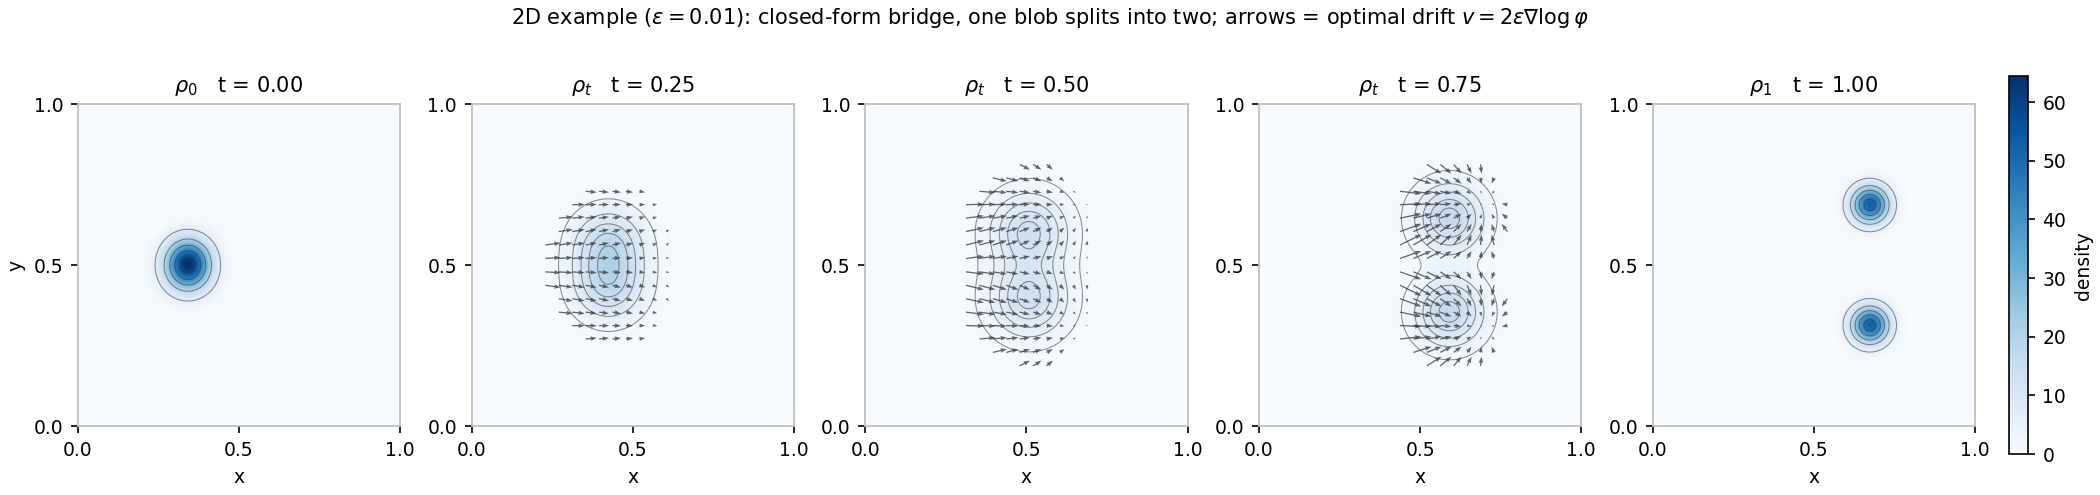
\includegraphics[width=\textwidth]{figures/mixture_sb_2d.png}\\[2pt]
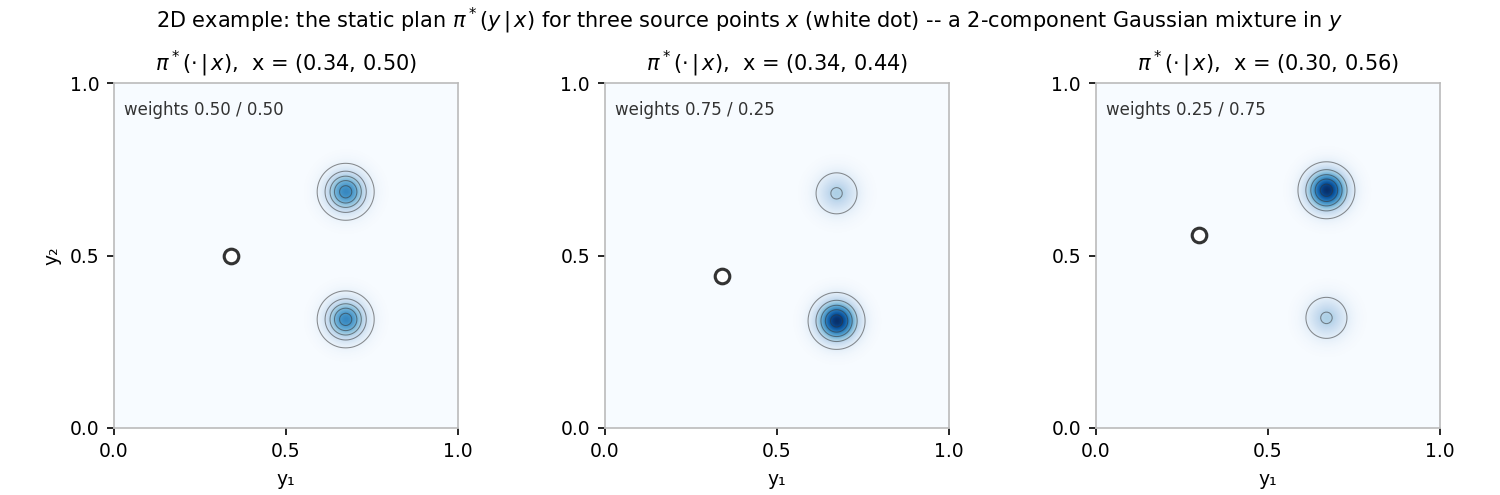
\includegraphics[width=0.8\textwidth]{figures/mixture_sb_2d_plan.png}
\caption{2D example, all from the closed form (no solver run). Top: $\rho_0$, three
intermediate $\rho_t$ with the optimal drift \eqref{eq:mixv} as arrows, and $\rho_1$;
shared colour scale, contours at 10--90\% of each panel's own peak. The bridge spreads
to roughly twice its endpoint width at $t=\tfrac12$ (the $\eps$ bulge of
Sec.~\ref{sec:gaussian}) and recondenses. Bottom: the static plan
$\pi^\ast(y\,|\,x)$ for three source points: a two-component Gaussian mixture in $y$
whose weights tilt toward the nearer target (this is the paper's Prop.~3.3 object,
and what its ``sampler'' draws from).}
\label{fig:mix2d}
\end{figure}

\paragraph{Worked 3D example (two blobs go to three).}
$\eps=0.005$, $\hat\varphi_0=\tfrac12\mathcal N((0.30,0.35,0.50),0.05^2I)+\tfrac12\mathcal N((0.30,0.65,0.50),0.05^2I)$,
$\varphi_1=\tfrac13\sum_{n=1}^3\mathcal N(b_n,0.04^2I)$ with
$b_1=(0.70,0.30,0.35)$, $b_2=(0.70,0.70,0.35)$, $b_3=(0.70,0.50,0.70)$
(\code{example\_split\_3d}). The branch-mass matrix is
\[
  \omega=\begin{pmatrix}0.391&0.006&0.103\\0.006&0.391&0.103\end{pmatrix}
  \quad(\text{rows: source blobs; columns: targets } b_1,b_2,b_3),
\]
i.e.\ each source sends $78\%$ of its mass to the nearest target, $21\%$ up to the
shared target $b_3$, and $1\%$ across to the far one. $\rho_0$ has six Gaussian
components but only two visible blobs (std $0.045$, centres $x\approx0.37$);
$\rho_1$ has three visible blobs (std $0.038$, $x\approx0.655$). Mass inside the box
$\ge1-2\cdot10^{-8}$; kinetic energy $0.0640$. The $1\%$ cross branch is a good
stress test: it is a low-density bridge between two far blobs, exactly where a
positivity-challenged scheme or an under-converged LADMM goes wrong first
(Fig.~\ref{fig:mix3d}).


\begin{figure}[htbp]\centering
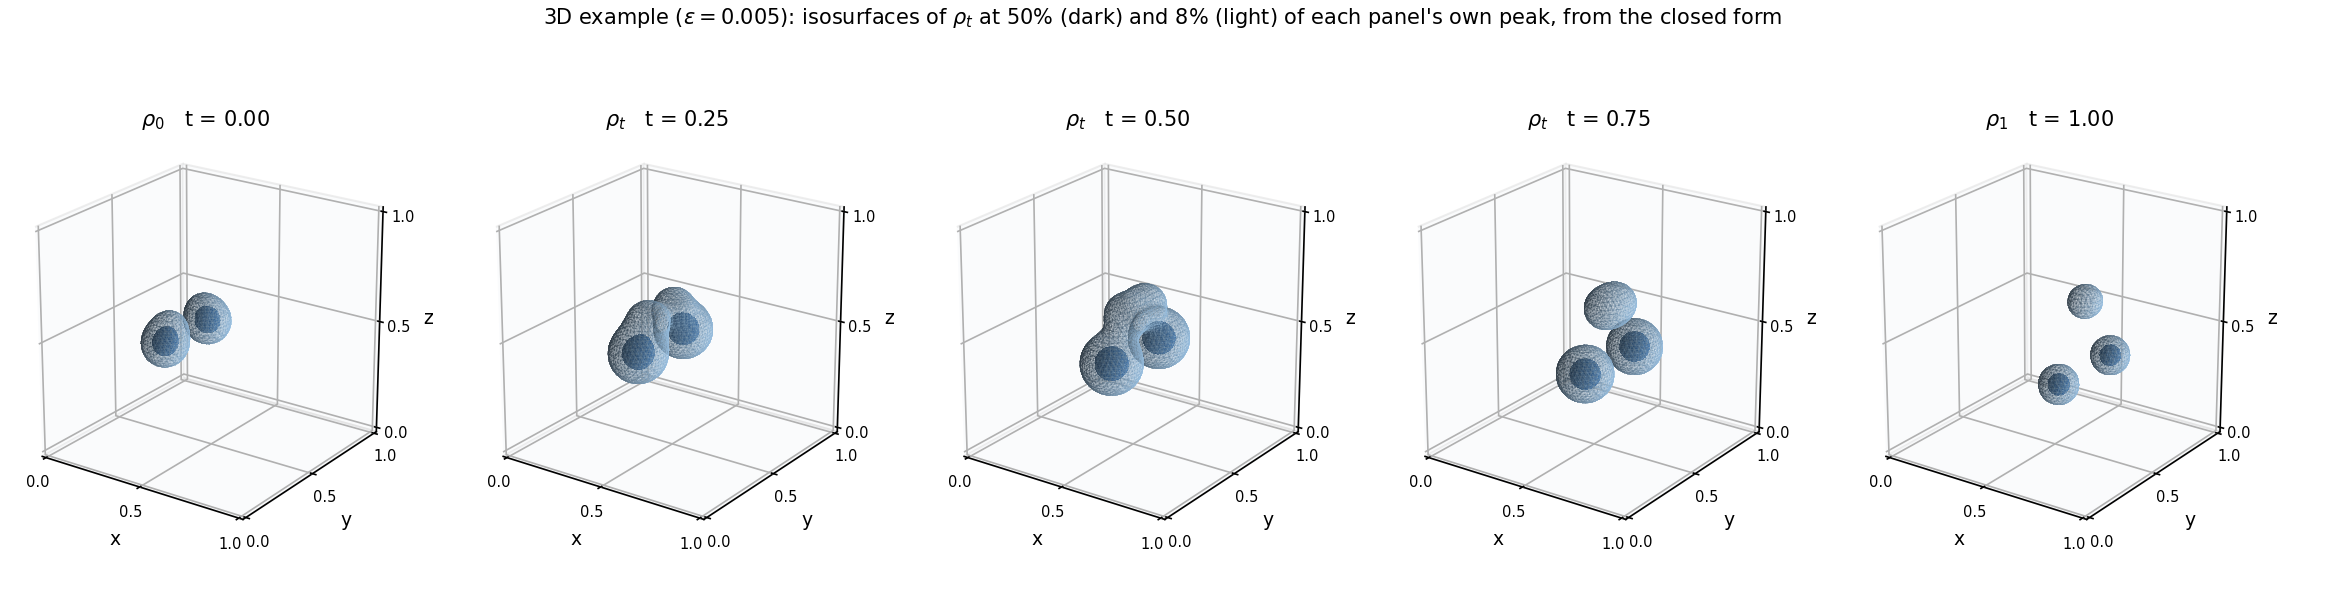
\includegraphics[width=\textwidth]{figures/mixture_sb_3d_iso.png}\\[2pt]
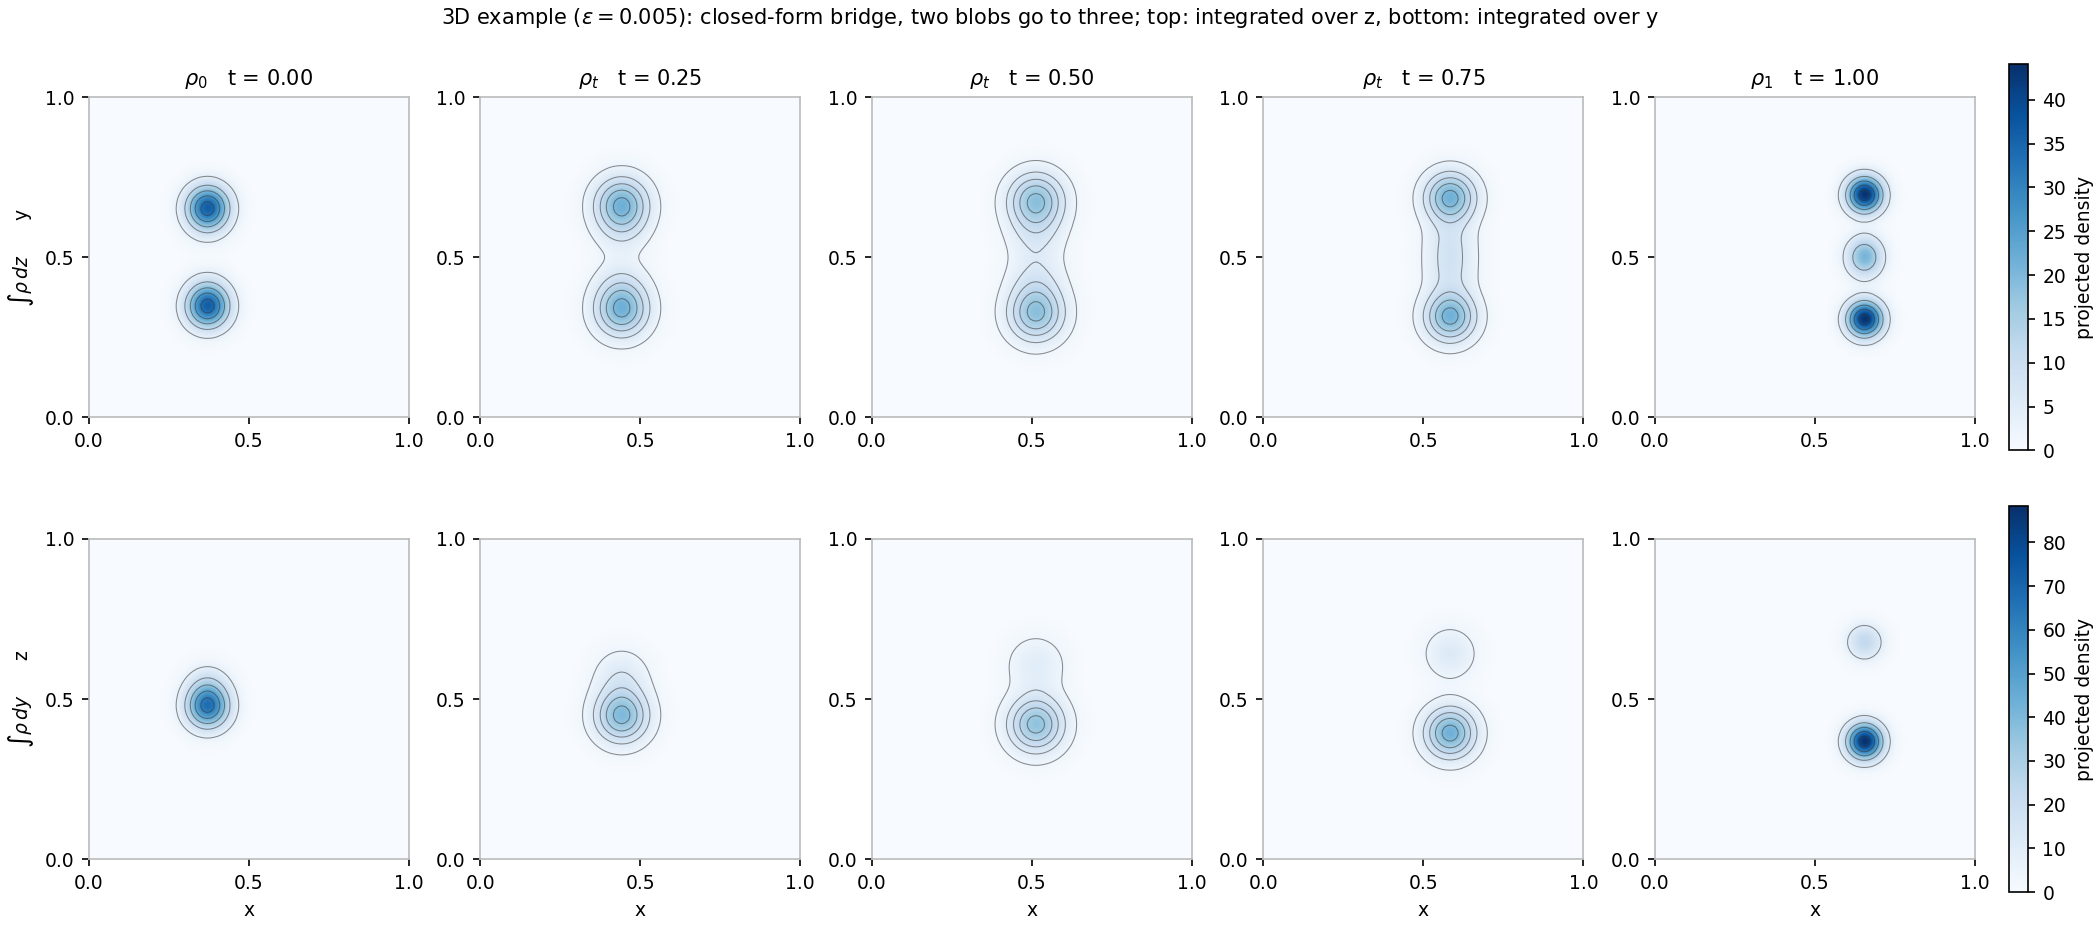
\includegraphics[width=\textwidth]{figures/mixture_sb_3d.png}
\caption{3D example from the closed form. Top row: isosurfaces of $\rho_t$ at 50\%
(dark) and 8\% (light) of each panel's own peak. Lower rows: projections of $\rho_t$
onto the $x$--$y$ plane and the $x$--$z$ plane. Two blobs become three; the third target
at $z=0.70$ receives $21\%$ of the mass and is visible from $t=0.5$ in the bottom
row, while the faint $x$--$y$ band between the two main blobs at $t=0.75$ is the
$1\%$ cross branch plus the shared branch.}
\label{fig:mix3d}
\end{figure}

\paragraph{Worked 2D example along the paper's route: a fixed, non-mixture $\rho_0$.}
The closed-form variant above only produces Gaussian-mixture marginals. To see
whether the construction transfers to a genuinely different $\rho_0$, the paper's
own route was followed, with one numerical step. Code:
\code{python/shared/paper\_route\_sb.py}, example \code{example\_ring\_to\_two\_2d}.
The six objects are obtained in this order (Fig.~\ref{fig:ringbuild}):
\begin{enumerate}[leftmargin=1.6em, itemsep=1pt]
  \item \emph{Choose} $\varphi_1(y)=\tfrac12\mathcal N(y|(0.70,0.30),0.04^2I)+\tfrac12\mathcal N(y|(0.70,0.70),0.04^2I)$. This is the paper's LSE-quadratic potential $g^\ast=\sigma^2\log\varphi_1$ with $A_n\succ0$.
  \item \emph{Closed form:} $\varphi(t,x)=\sum_n w_n\mathcal N(x|b_n,Q_n+2\eps(1-t)I)$, the backward heat flow. At $t=0$ this is $\varphi_1$ blurred by variance $2\eps$, a smooth two-lobed modulation; it is also $Z(x)$ in \eqref{eq:cond} up to a constant.
  \item \emph{Fix} $\rho_0$: a smooth ring, $\rho_0\propto\exp\bigl(-(|x-c|-r)^2/2w^2\bigr)$ with $c=(0.35,0.50)$, $r=0.12$, $w=0.025$, normalized on the grid. It is not a Gaussian mixture.
  \item \emph{Forced:} $\hat\varphi_0=\rho_0/\varphi(0,\cdot)$. There is no freedom here; this is what makes the $x$-marginal come out as $\rho_0$. In the paper this factor is never written down because the sampler never needs it. Here it is a crescent: the part of the ring facing away from the targets, where $\varphi(0,\cdot)$ is smallest.
  \item \emph{The one numerical step:} $\hat\varphi(t,\cdot)=\mathcal N(0,2\eps tI)\ast\hat\varphi_0$, the forward heat flow. Since the target points form a tensor grid and the kernel is separable, this is $K_x F K_y^{\top}$ with $F$ the values of $\hat\varphi_0$ on a fine $n_f\times n_f$ grid and $K_x$ the $n\times n_f$ matrix of 1D Gaussian weights times the cell width. Midpoint quadrature of a smooth Gaussian integrand is spectrally accurate: against $n_f=1024$, the $n_f=128$ result differs by $1.4\cdot10^{-8}$ (relative to the peak) at the smallest time the solver needs, $t=1/32$, and $n_f=512$ by $2\cdot10^{-10}$; at $t\ge\tfrac12$ all are below $10^{-9}$.
  \item \emph{Products:} $\rho_t=\varphi(t,\cdot)\,\hat\varphi(t,\cdot)$ (no constant, since $\int\rho_0=1$), $\rho_1=\varphi_1\hat\varphi(1,\cdot)$, and $v=2\eps\nabla\log\varphi(t,\cdot)$ from step 2, closed form and independent of $\rho_0$; $m=\rho_tv$.
\end{enumerate}
Checks, as for the mixture case: $\int_{[0,1]^2}\rho_t=1$ to $8\cdot10^{-7}$ at all $t$
(the deficit is the mass that diffuses past the walls on $\R^2$ and comes back);
$\rho_1$ equals the paper's definition $\int\rho_0(x)\pi^\ast(y|x)\,dx$ by direct
quadrature to $3\cdot10^{-16}$; the finite-difference residual of
$\partial_t\rho+\dv(\rho v)-\eps\Delta\rho$ is $1.9\cdot10^{-3},4.7\cdot10^{-4},
1.2\cdot10^{-4}$ on $200^2,400^2,800^2$ grids at $t=\tfrac12$, i.e.\ $O(h^2)$, and
likewise at $t=0.1$ and $0.9$. Kinetic energy $0.0911$. Peak density $21$ at $t=0$,
$10$ at $t=\tfrac14$, $52$ at $t=1$. Building the full staggered-grid reference at
$32^3$ takes $0.3$\,s.

\begin{figure}[htbp]\centering
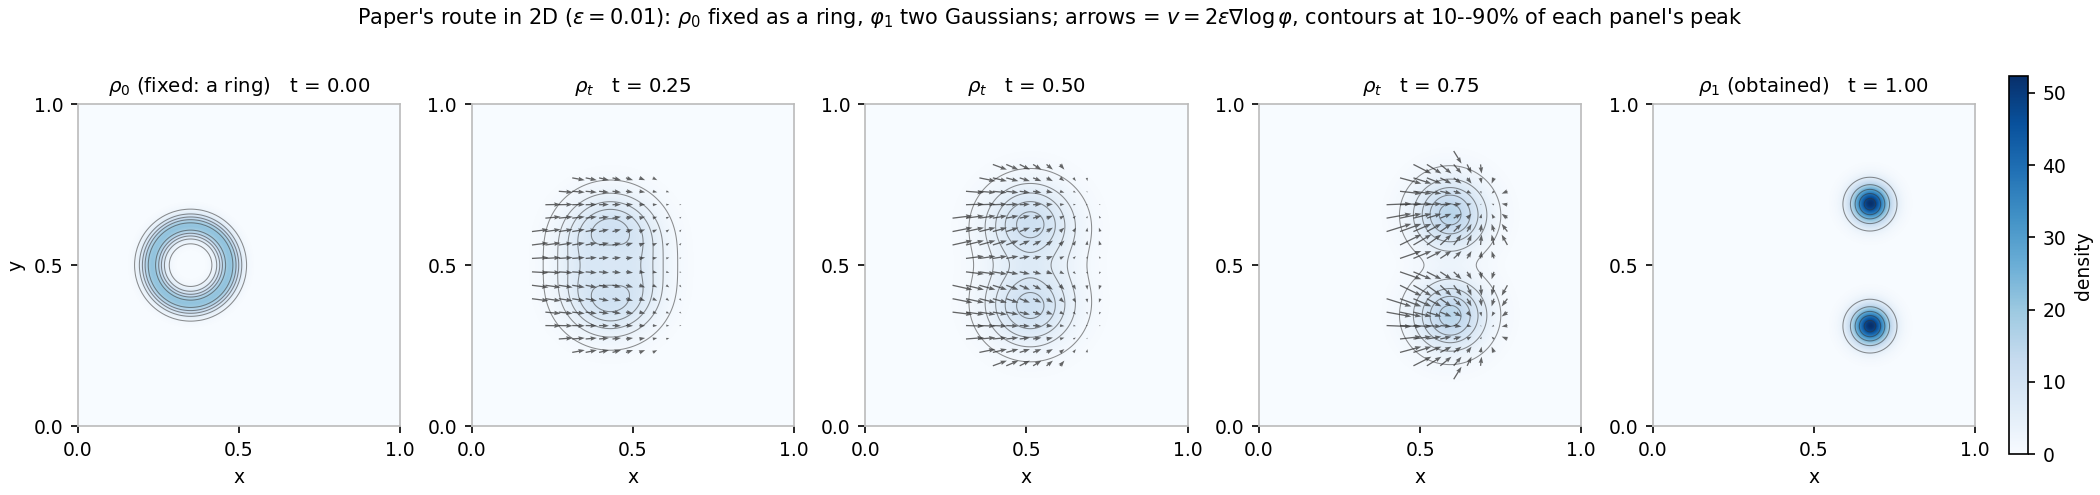
\includegraphics[width=\textwidth]{figures/ring_sb_2d.png}
\caption{The paper's route in 2D: $\rho_0$ fixed as a ring, $\varphi_1$ two Gaussians.
Everything else is derived. The ring fills in and stretches toward the targets by
$t=\tfrac14$, is a two-lobed cloud at $t=\tfrac12$, and arrives as two Gaussian-looking
blobs. Arrows: $v=2\eps\nabla\log\varphi$. Shared colour scale, contours at
$10$--$90\%$ of each panel's own peak.}
\label{fig:ring}
\end{figure}
\begin{figure}[htbp]\centering
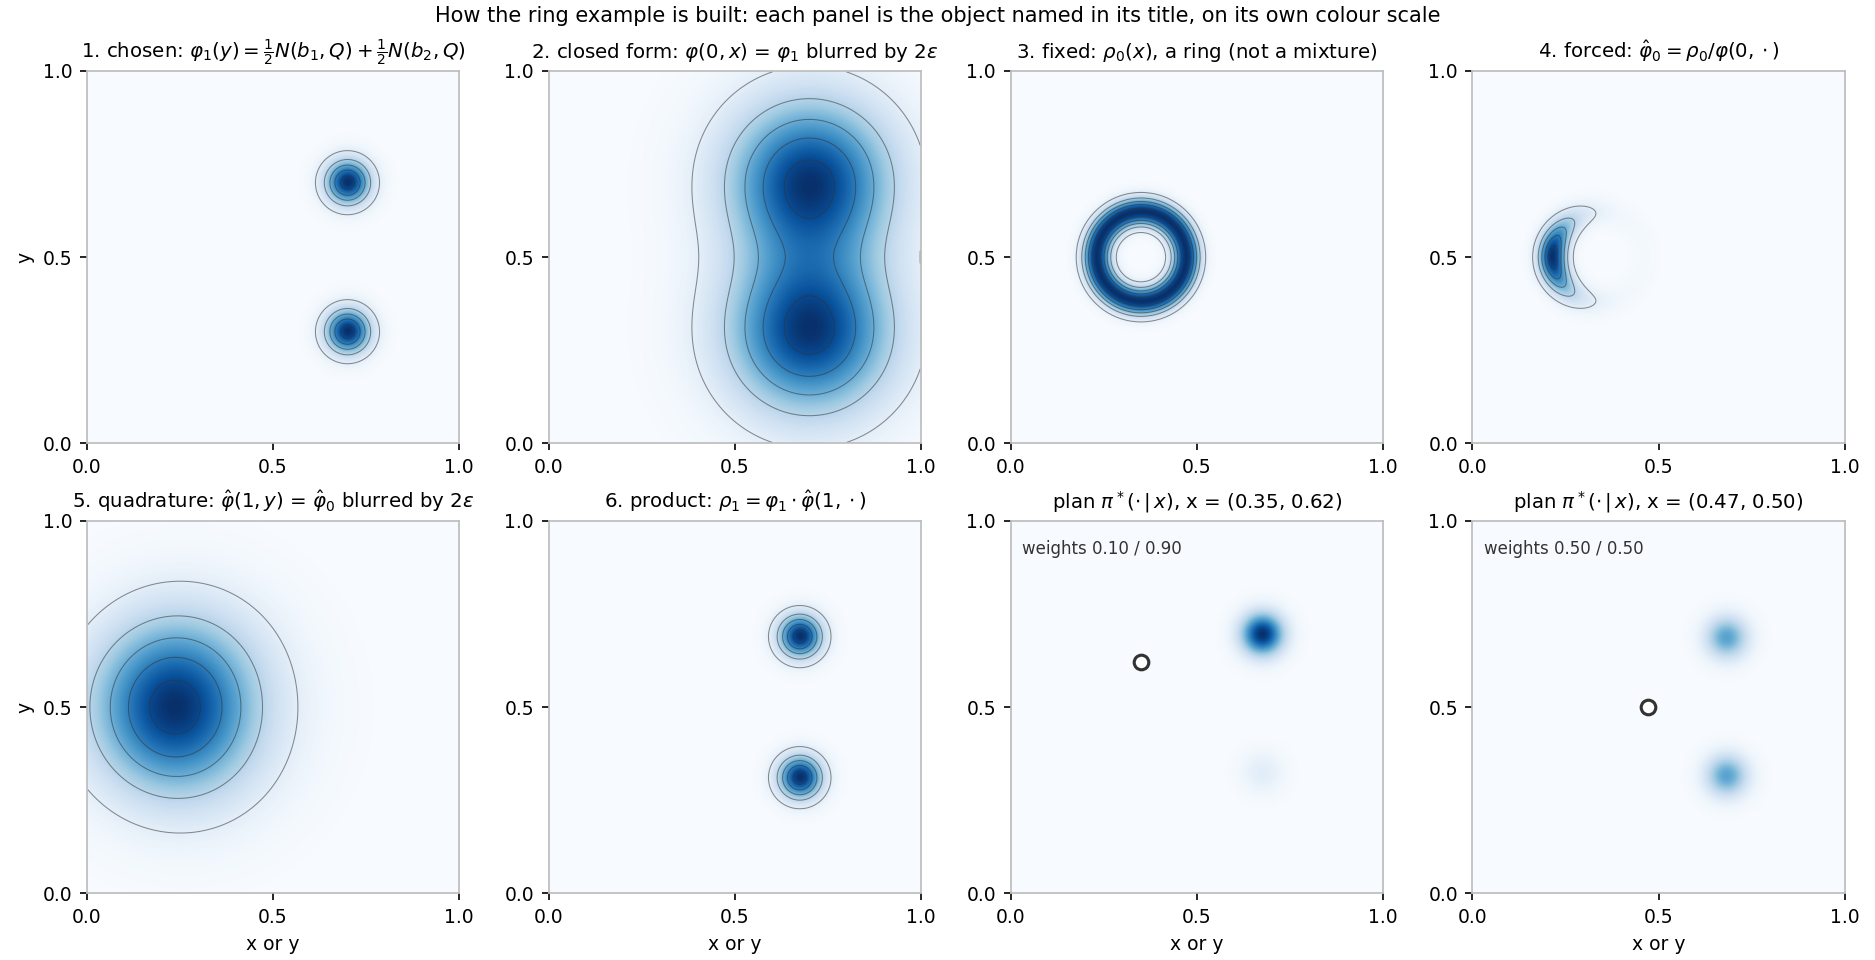
\includegraphics[width=\textwidth]{figures/ring_sb_2d_construction.png}
\caption{How the ring example is built, numbered as in the text. Top: the chosen
factor $\varphi_1$, its closed-form blur $\varphi(0,\cdot)$, the fixed $\rho_0$, and the
forced factor $\hat\varphi_0=\rho_0/\varphi(0,\cdot)$, a crescent on the side of the
ring away from the targets. Bottom: the one quadrature, $\hat\varphi(1,\cdot)$; the
product $\rho_1$; and the static plan $\pi^\ast(y|x)$ for two source points on the
ring, each a two-Gaussian mixture in $y$ whose weights depend on where $x$ sits on
the ring ($0.10/0.90$ at the top of the ring, $0.50/0.50$ on the symmetry line).}
\label{fig:ringbuild}
\end{figure}

\paragraph{Does this transfer to verifying the grid solver?}
Yes, with the following accounting. The solver returns $\rho$ on cell centres at
$k\,dt$ and $m$ on faces at $(k-\tfrac12)dt$; \code{staggered\_reference} evaluates
steps 2, 5 and 6 at exactly those points, so the comparison is pointwise, with no
interpolation of the reference. The reference error budget is: quadrature in
step~5, $\le10^{-9}$ for $n_f\ge256$; the $\R^2$-versus-box mismatch, bounded by the
tail mass ($8\cdot10^{-7}$ here, set by how far the support sits from the walls);
and nothing else, since steps 1--4 and 6 are closed form. Both are far below the
$O(h^2)$ discretization error one is measuring ($10^{-2}$--$10^{-3}$ for
$n=32$--$128$). In 3D step~5 becomes three tensor contractions,
$\hat\varphi(t)=F\times_1K_x\times_2K_y\times_3K_z$, with $F$ on a $256^3$ grid;
cost $O(n\,n_f^3)$ per time slice, seconds on a GPU, so a $96^4$ reference is cheap.
What one gives up relative to the mixture case is the readable branch-mass table
and the closed-form $\rho_1$; what one gains is complete freedom in $\rho_0$ (any
smooth positive density that is small at the walls) while $v$ stays closed form.
Two practical rules. Keep $\rho_0$ smooth on the scale of $\sqrt{2\eps\,dt}$, the blur
at the first time step, or the forced factor $\hat\varphi_0$ will be rough. And choose
$\varphi_1$ so that $\varphi(0,\cdot)$ does not vary wildly across the support of
$\rho_0$, or $\hat\varphi_0$ concentrates on a sliver of it: here $\varphi(0,\cdot)$
varies by a factor 261 over the ring, which already turns the ring into the
crescent of Fig.~\ref{fig:ringbuild}; a larger $\eps$ or targets closer to $\rho_0$
reduce this. If the wall truncation ever matters, replace the Gaussian kernels in
steps 2 and 5 by the Neumann heat kernel of the box (a cosine series, or the method
of images); then the reference satisfies the no-flux condition exactly.

\paragraph{Caveats and knobs.}
\begin{itemize}
  \item The paper allows $A_n$ with eigenvalues in $(-1,0)$ (a locally
        \emph{repulsive} potential). Those are not Gaussian mixtures and are excluded
        here; the price is that $\rho_1$'s modes are always blobs around the $b_n$.
  \item Blob positions are pulled toward the other side: $c_{in}(0)$ lies between
        $a_i$ and $b_n$, more so for larger $\eps$ or wider $P_i$. Keep every
        $c_{in}(t)$ at least $4$--$5$ standard deviations of $C_{in}(t)$ inside the
        box; $C_{in}(t)$ is largest near the middle of $[0,1]$ in $t$.
  \item The mass split $\omega_{in}$ is an output. To force a given split, tune
        $u_i,w_n$ (they enter $\omega$ linearly) rather than the geometry.
  \item The same object with $I=N=1$ and unequal $P\neq Q$ is an unequal-covariance
        Gaussian bridge, an independent check on Sec.~\ref{sec:gaussian}.
\end{itemize}
Effort: low (the closed form is written down; no solver runs yet). Paper value:
good; multimodal exact references are novel in the grid-solver literature.

\subsection{Reflected SB theory (matches the no-flux walls)}

Caluya and Halder, ``Reflected Schr\"odinger Bridge: Density Control with Path
Constraints'', ACC 2021, arXiv:2003.13895: SB with reflecting boundaries. The
forward--backward PDE system has a no-flux Neumann condition on the forward factor
and an oblique Neumann condition on the backward factor. Useful to cite as the exact
continuous problem the discretization targets, and to justify tests where mass does
touch the walls (e.g.\ uniform $\to$ bump inside the box).

\section{Application problems}
\label{sec:applications}

\subsection{Cosmology: Lagrangian reconstruction (MAK) as dynamic OT}
\label{sec:cosmo}

Strongest narrative, with a boundary-condition mismatch to handle.

\paragraph{Literature.} Frisch, Matarrese, Mohayaee, Sobolevski, Nature 417:260
(2002); Brenier, Frisch, H\'enon, Loeper, Matarrese, Mohayaee, Sobolevskii,
``Reconstruction of the early Universe as a convex optimization problem'', MNRAS
346:501 (2003) (MAK; uniqueness for convex bounded domains); L\'evy, Mohayaee, von
Hausegger, MNRAS 506:1165 (2021), fast semi-discrete OT; von Hausegger, L\'evy,
Mohayaee, PRL 128:201302 (2022), BAO via semi-discrete OT; Nikakhtar, Sheth, L\'evy,
Mohayaee, PRL 129 (2022), OT reconstruction of BAO; Nikakhtar, Padmanabhan, L\'evy,
Sheth, Mohayaee, arXiv:2307.03671 (redshift space); arXiv:2606.01529 (primordial
non-Gaussianity). The problem is exactly displacement interpolation from a uniform
initial density to the $z=0$ density (Zel'dovich approximation $\Leftrightarrow$
quadratic-cost OT).

\paragraph{Schr\"odinger-bridge version.} The survey found \emph{no} paper doing an
entropic or SB cosmological reconstruction (searches for ``Schr\"odinger
bridge/problem'' with cosmology return only the unrelated Schr\"odinger--Poisson
method and Bunne-style SB theory). A 3D SB reconstruction with $\eps$ read as a small
velocity-dispersion / multistreaming smoothing would be a genuinely new, if modest,
contribution; the physical meaning is heuristic, so say so rather than claim it.

\paragraph{Boundary conditions.} All simulation tests use a periodic box (Brenier et
al.\ 2003; L\'evy et al.\ 2021; Nikakhtar et al.). Observational applications are
not periodic: Lavaux, Mohayaee, Colombi, Tully, Bernardeau, Silk, MNRAS 2008, pad a
$100\,h^{-1}$Mpc-deep 2MRS volume with a homogeneous particle distribution and trust
only the inner $60\,h^{-1}$Mpc. Practical recipe for our box: take a sub-cube, pad by
a margin at least the typical displacement (about $10\,h^{-1}$Mpc at $z=0$), and
evaluate only the interior; no-flux is then a controlled approximation.
Alternatively multiply by a smooth window. Flag this in the paper.

\paragraph{Data.} CAMELS Multifield Dataset (CMD), Villaescusa-Navarro et al., ApJS
259:61 (2022): 3D grids of $M_{\rm tot}$, $M_{\rm cdm}$, $M_{\rm gas}$, etc.\ at
$128^3$, $256^3$, $512^3$ voxels over $(25\,h^{-1}\mathrm{Mpc})^3$ at redshifts
$0, 0.5, 1, 1.5, 2$; float32 \code{.npy}, 8\,MB per $128^3$ grid; periodic;
\url{https://camels-multifield-dataset.readthedocs.io} (Globus / binder / URL).
Quijote (Villaescusa-Navarro et al.\ 2020): 3D density fields at $64$--$512^3$ over
$(1000\,h^{-1}\mathrm{Mpc})^3$, CIC/PCS, \code{.npy},
\url{https://quijote-simulations.readthedocs.io/en/latest/df.html}. A $128^3$ CMD
$z=2\to0$ pair downsampled to $96^3$ (or $z=1\to0$ to keep displacements small) is a
ready-made problem. Uniform $\to z=0$, the MAK problem proper, also works: the
initial density is uniform by construction.

\paragraph{What $\rho_0$ and $\rho_1$ are on a grid.}
Brenier et al.\ discretize into $N$ equal point masses because their solver is an
assignment algorithm: the $N$ particles of an $N$-body simulation at $z=0$ are
matched to the $N$ sites of a regular Lagrangian lattice, which is the uniform
initial state. The grid version of the same two measures is:
\begin{itemize}
  \item $\rho_0(q)\equiv1$ (in units of the mean density) on the Lagrangian grid
        $q\in[0,L]^3$. At decoupling the fluctuations are $\delta\sim10^{-5}$, so
        ``uniform'' is exact for every purpose here. This is the continuum limit of
        Brenier's lattice of equal masses; the lattice spacing is what they call the
        mesh ($6.25\,h^{-1}$Mpc in their tests) and plays the role of our cell size.
  \item $\rho_1(x)$ on the Eulerian grid $x\in[0,L]^3$: the $z=0$ mass deposited on
        the cells by cloud-in-cell (CIC) assignment, divided by the mean, so that
        $\int\rho_1=\int\rho_0$ automatically. The public density fields (Quijote,
        CAMELS) are exactly this object; from a particle snapshot it is one
        \code{np.add.at}. A floor of a few percent of the mean for empty voids is the
        only preprocessing.
\end{itemize}
The dimension is three: the physical problem is 3D, the data are 3D, and the
reconstruction literature is 3D. A 2D version is legitimate for development only
if it is generated as a 2D flow (a 2D potential and 2D displacement), because a 2D
slice of a 3D flow does not conserve mass within the slice. The quadratic cost in
comoving coordinates and growth-factor time $t=D(z)/D(0)$ are the same in any
dimension.

\paragraph{The problem as the solver sees it (Fig.~\ref{fig:mak}).}
Fig.~\ref{fig:mak} shows a realization built without any download
(\code{python/shared/zeldovich.py}): a Gaussian random linear density field with a
BBKS $\Lambda$CDM-like spectrum ($\Gamma=0.21$, $n_s=0.96$, $\sigma_8=0.8$) is
synthesized in the cosine basis of a $512\,h^{-1}$Mpc box, so the displacement
potential is even about every wall and the Zel'dovich displacement
$\Psi=-\nabla\Phi$, $\nabla^2\Phi=\delta$, has zero normal component on the walls.
$128^3$ particles are placed on the Lagrangian grid and moved to $x=q+D\,\Psi(q)$,
and $\rho_1$ is their CIC deposit on $96^3$ cells of $5.3\,h^{-1}$Mpc, the resolution
the solver can afford. Numbers for this realization at $D=1$ ($z=0$): rms
displacement $9.5\,h^{-1}$Mpc, i.e.\ $1.8$ cells, maximum $33\,h^{-1}$Mpc; $\rho_1$
ranges from empty cells to $29\times$ the mean, with $2.2\%$ of cells below $0.1$
and $1.1\%$ above $5$; $15\%$ of Lagrangian cells are shell-crossed
($\det(I+\nabla\Psi)\le0$). At $D=0.5$ ($z\approx1$) the range is $0.05$--$8.7$ with
$0.07\%$ shell-crossed cells, and at $D=0.3$ ($z\approx2$) it is $0.2$--$4.7$ with
none.

\begin{figure}[htbp]\centering
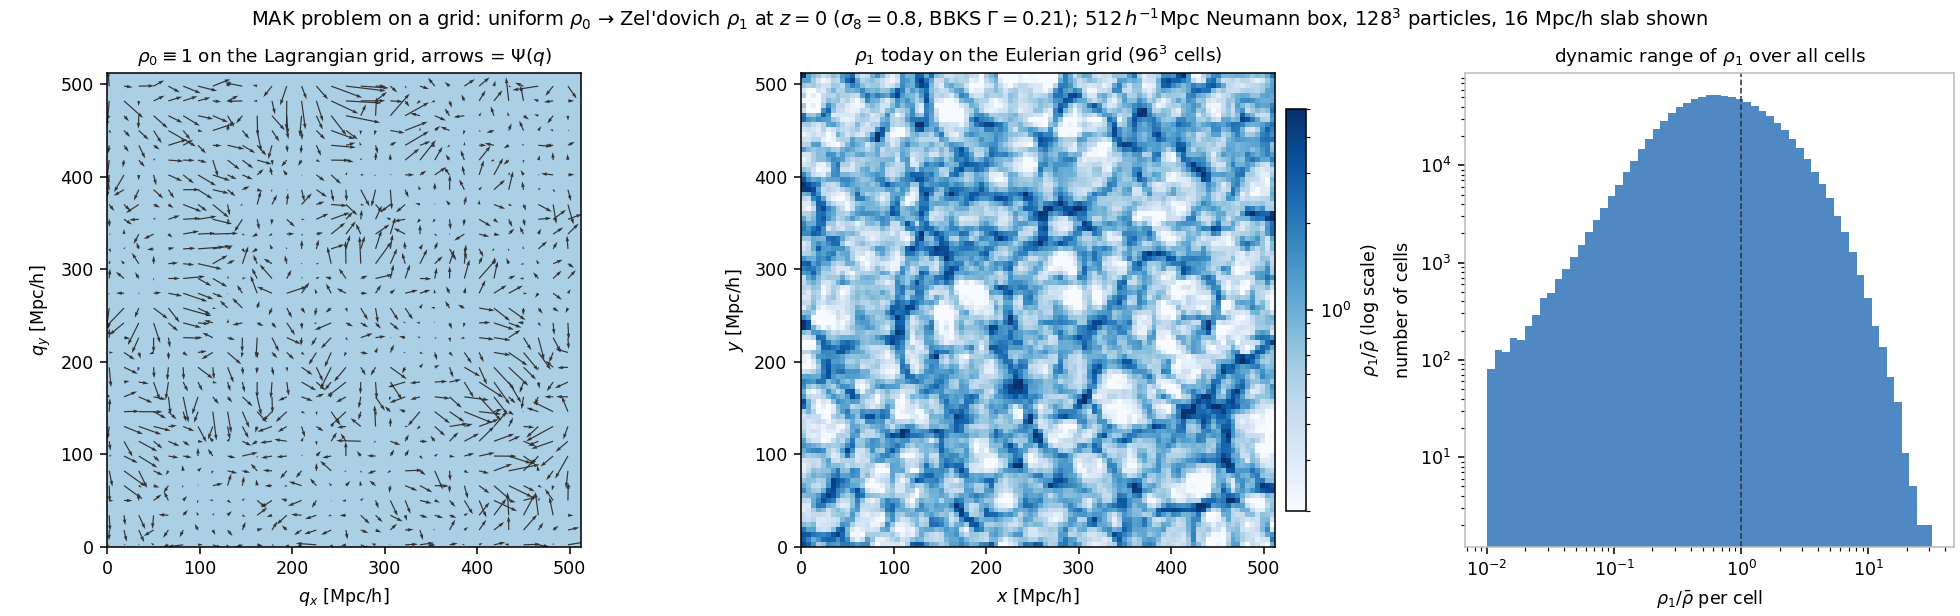
\includegraphics[width=\textwidth]{figures/mak_rho0_rho1.png}
\caption{The MAK problem on the solver's grid. Left: $\rho_0\equiv1$ on the
Lagrangian grid, with the Zel'dovich displacement $\Psi(q)$ of a $16\,h^{-1}$Mpc slab
drawn as arrows; this field is the \emph{answer} the reconstruction has to recover.
Middle: $\rho_1$, the same slab today, on $96^3$ cells, log colour scale: the
arrows converge onto the filaments and knots and diverge out of the voids. Right:
the histogram of $\rho_1$ over all cells, the dynamic range the prox has to handle.}
\label{fig:mak}
\end{figure}

\paragraph{What the figure means physically.} Every arrow on the left is the
comoving path of a parcel of dark matter from the nearly uniform early Universe to
where it sits today; in the Zel'dovich approximation the parcels move in straight
lines at constant comoving velocity, with the growth factor $D$ as the clock, and
$\Psi$ is a gradient field. Where arrows converge, sheets form first (``pancakes''),
then filaments where sheets intersect, then the knots that host clusters; where
they diverge, voids empty out. The reconstruction problem inverts the middle panel
into the left one: given only today's density, find the gradient displacement that
produced it. Brenier's theorem says this inverse is unique as long as the map is
the gradient of a convex potential, i.e.\ before shell crossing, and that it is the
quadratic-cost optimal transport from $\rho_0$ to $\rho_1$. In solver terms:
$\rho(t,\cdot)$ at $t=D(z)/D(0)$ is the density at redshift $z$, and the velocity
$m/\rho$ at $t\to0$, read on the uniform grid, \emph{is} the reconstructed
$\Psi(q)$, which is also the peculiar velocity field up to the factor $fHa$. The
$15\%$ shell-crossed cells at $z=0$ are where multistreaming has erased the inner
velocity structure; this is the one place where a small $\eps$ has a plausible
reading, as a velocity dispersion, and the reason the exact-answer test should be
run at $D\approx0.3$--$0.5$ where no crossing has occurred and the arrows in the left
panel are the exact solution.

\paragraph{Sanity check.} Compare the OT displacement field against the true
Lagrangian displacements available from particle IDs (needs the raw snapshots, on the
CAMELS Globus), or at least against the MAK / semi-discrete solution (L\'evy's code is
public). The dynamic range at $z=0$ is huge (voids $\sim0.1$, filaments $>100\times$
the mean): expect stiffness, and consider a smoothing scale as Nikakhtar et al.\ do.

Effort: moderate. Paper value: high; a recognizable application with a large
literature and a periodic-versus-no-flux discussion reviewers will find honest.

\subsection{Cryo-EM density maps (EMDB)}
\label{sec:cryoem}

The best real-data fit to the box: maps are already on uniform Cartesian grids with
zero density at the box edges (ideal for no-flux), nonnegative after thresholding,
mass renormalizable; a conformational change is a physically meaningful displacement
interpolation.

\paragraph{Literature doing this with static entropic OT.} Ecoffet, Poitevin, Dao
Duc, ``MorphOT: transport-based interpolation between EM maps with UCSF ChimeraX'',
Bioinformatics 36:5528 (2020), bioRxiv 10.1101/2020.09.08.286302; Ecoffet et al.,
``Application of transport-based metric for continuous interpolation between cryo-EM
density maps'', AIMS Mathematics 7(1) (2022), PMC9377683: entropic $W_2$ barycenters
via Gaussian convolution (Solomon et al.), tested at $60^3$, $120^3$, $240^3$,
default downsampling to $60^3$, $\gamma=1$, at most 1500 iterations; they assume equal
mass and list unbalanced OT as future work. Alignment: Riahi, Woollard, Poitevin,
Condon, Dao Duc, ``AlignOT'', IEEE TCBB 2023 (arXiv:2210.09361); Riahi et al.,
``EMPOT'', arXiv:2311.00850; PRX Life 3:023003 (2025). Zelesko, Moscovich, Kileel,
Singer, ISBI 2020, ``Earthmover-based manifold learning'', used a simulated
ATP-synthase rotary dataset (public availability not verified).

\paragraph{Concrete pairs.} Used by MorphOT: the Mm-cpn group II chaperonin,
EMD-5137 (wild-type closed, 4.3\,\AA) and EMD-5139 (wild-type open, 8\,\AA), Zhang et
al., Nature 463:379 (2010); also the lidless EMD-5138 / EMD-5140. Same particle, same
lab, same box: align rigidly (AlignOT / ChimeraX) and resample to $64$--$96^3$.
Alternatively the E.\ coli ATP synthase rotational states EMD-20006 / EMD-20008
(Sobti et al., eLife 2019), three rotary states of the same complex.

\paragraph{Reference.} MorphOT's Sinkhorn barycenters at the same $\gamma$ (they use
an $\R^3$ Gaussian kernel, not Neumann; the difference should be negligible with
zero-padded maps), plus our own DCT-Sinkhorn (Section~\ref{sec:dctsinkhorn}). Our
dynamic solver adds what they lack: momentum / velocity fields (which map to residue
motions) and an $\eps$ that plays the role of their blur.

Effort: low to moderate (download from \url{https://www.ebi.ac.uk/emdb/}, threshold,
align, resample). Paper value: high; ``static barycenter vs.\ dynamic bridge on
EMD-5137 $\to$ 5139'' is a clean figure.

\paragraph{Can it be run? Yes, 3D, and it is the cleanest real-data fit.} An EMDB
entry is a single-precision 3D array on a cubic voxel grid (typically $1$--$4$\,\AA\
per voxel, $200$--$400$ voxels per side) with the particle centred and solvent at the
edges. $\rho_0$ and $\rho_1$ are two maps of the same complex in two conformations:
threshold at zero (map noise is signed), optionally mask the solvent, align rigidly,
resample both to $96^3$, and normalize. Equal mass is physically exact, since it is
the same molecule, and zero density at the walls is automatic.
Fig.~\ref{fig:appcryo} shows a phantom with the architecture of the MorphOT pair
EMD-5137/5139: two stacked eight-fold rings of subunits, each with an apical ``lid''
domain that folds over the central cavity in the closed state and swings outward in
the open state. Interpretation: $\rho_t$ is the conformational transition path
between the two states, the quantity MorphOT produces as a static barycenter
sequence, and $m/\rho$ is the domain motion field, which can be read against the
atomic models fitted to each map (the lid domains should move outward and up, the
equatorial ring should barely move). \textbf{$\eps$ has no physical meaning as a
diffusion}; its honest reading is the resolution of the maps: a map at $8$\,\AA\ is a
sharper map blurred by a kernel of that width, so matching $\sqrt{2\eps}$ to the
lower of the two resolutions (here $8$\,\AA, about $1$--$2$ cells at $96^3$) makes
the bridge's blur commensurate with the data's, and MorphOT's $\gamma$ is the same
blur in their convention. The phantom's density spans zero to $42\times$ the mean
inside the particle envelope, so a floor in the solvent region is the only stiffness
precaution.
\begin{figure}[htbp]\centering
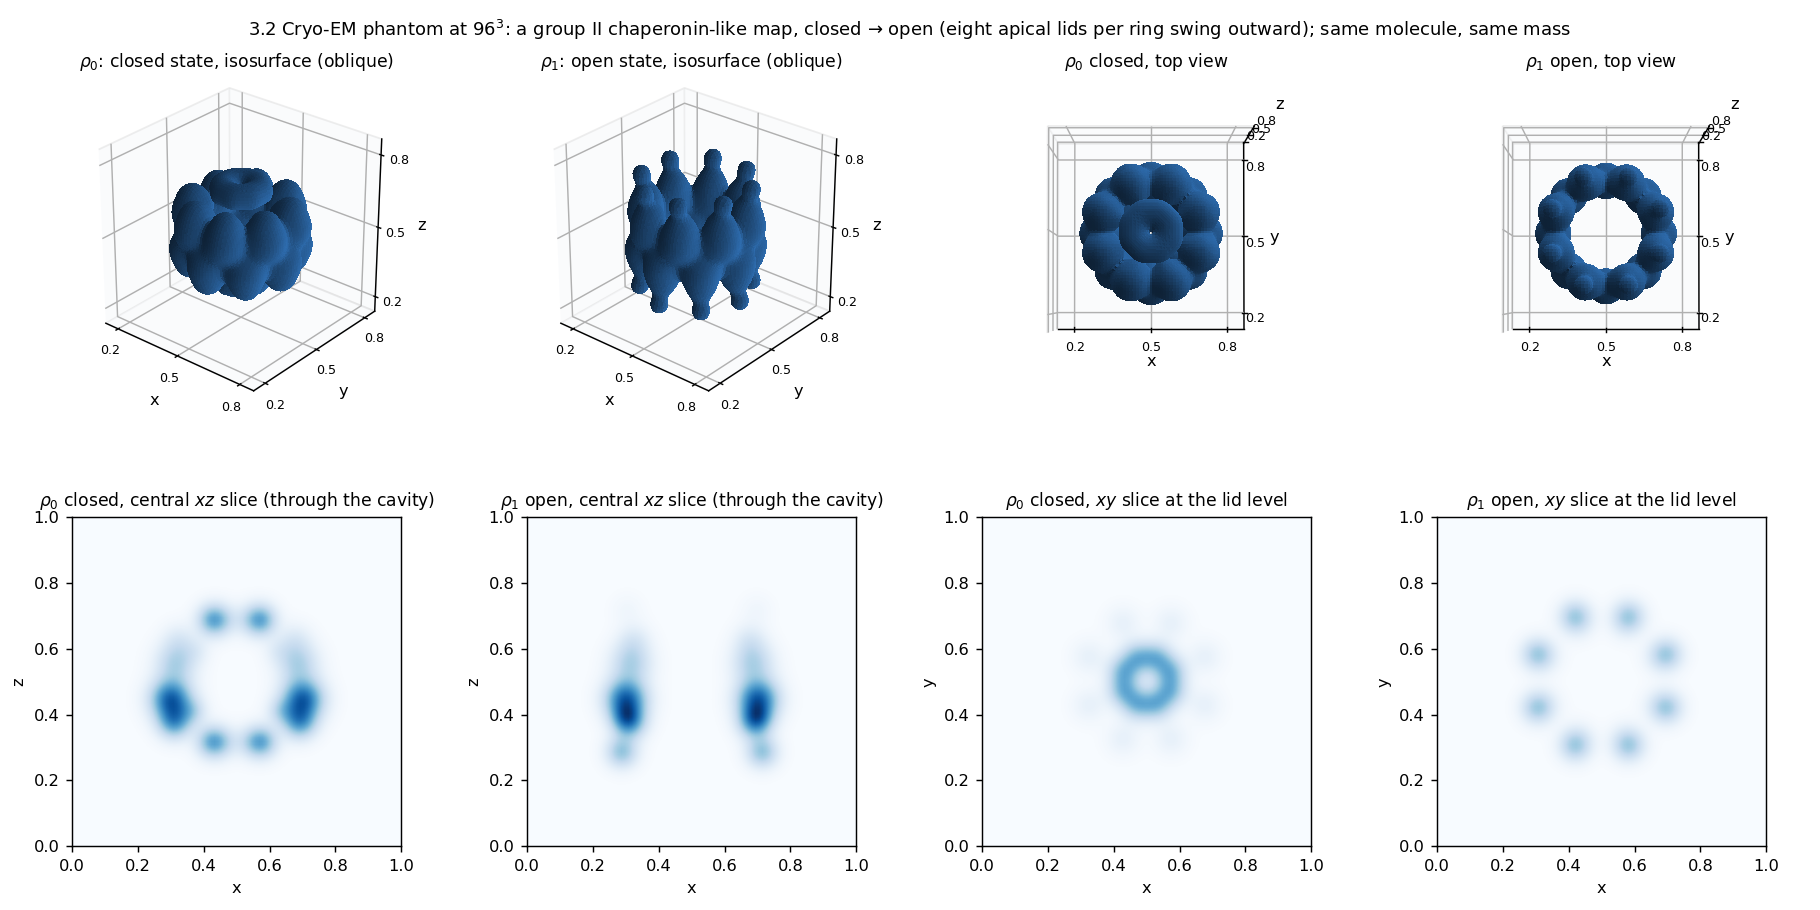
\includegraphics[width=\textwidth]{figures/app_cryoem.png}
\caption{Cryo-EM phantom at $96^3$. Top: isosurfaces at $25\%$ of the peak for the
closed ($\rho_0$) and open ($\rho_1$) states, oblique and from the top; the eight lids
of the upper ring close the cavity in $\rho_0$ and open into a flower in $\rho_1$.
Bottom: a central vertical slice through the cavity and a horizontal slice at the
lid level, same colour scale.}
\label{fig:appcryo}
\end{figure}

\paragraph{Smaller alternative: molecular electron densities.} Gaussian \code{.cube}
files are uniform grids (e.g.\ EDBench, arXiv:2505.09262, about 3.4M molecules with
cube files; QM9-derived densities at $256^3$ / 0.1\,bohr). A chemRxiv 2025 preprint,
``Electron Density Transport During Chemical Reactions'' (10.26434/chemrxiv, April
2025), already uses POT / Sinkhorn on cube densities along reaction paths. Two
snapshots of a reaction (reactant and product densities) have equal electron count,
so equal mass automatically: a tidy small problem. Effort: low. Paper value:
moderate, novel.

\subsection{Medical imaging}

\paragraph{OT in 3D registration.} Haker, Zhu, Tannenbaum, Angenent, IJCV 60:225
(2004), Monge--Kantorovich warping of 3D brain MRI. Chen, Elkin, Tannenbaum et al.,
``Visualizing fluid flows via regularized optimal mass transport with applications to
neuroscience'', J.\ Sci.\ Comput.\ (2023), and ``Unbalanced regularized optimal mass
transport with applications to fluid flows in the brain'', Sci.\ Rep.\ (2024),
\url{https://www.nature.com/articles/s41598-023-50874-y}: a Benamou--Brenier plus
diffusion (advection--diffusion) model, essentially our PDE, solved on cell-centred
grids of $50^3$ (synthetic) and $56\times106\times51$ (rat-brain DCE-MRI, glymphatic
tracer). This is the closest existing 3D application of our exact formulation, and
there the diffusion coefficient has physical meaning (tracer diffusivity). The rat
data do not appear to be public, but the model and grid sizes are a direct benchmark
to cite.

\paragraph{Datasets.}
\begin{itemize}
  \item DIR-Lab 4DCT (\url{https://www.dir-lab.com/}): 10 cases, 10 respiratory
        phases, about $1\times1\times2.5$\,mm, 300 landmark pairs between end-exhale
        and end-inhale, which give a sanity check on the transport map.
  \item Learn2Reg OASIS brain MRI (\url{https://learn2reg.grand-challenge.org/}): 416
        skull-stripped 1\,mm T1 scans cropped to $160\times224\times192$, with label
        maps for Dice checks.
  \item BrainWeb phantoms (\url{https://brainweb.bic.mni.mcgill.ca/}):
        $181\times217\times181$ at 1\,mm with ground-truth tissue classes.
  \item ACDC cardiac cine (Bernard et al., IEEE TMI 2018): in-plane 1.4--1.7\,mm but
        slices 5--8\,mm; anisotropic, a poor fit for a cubic grid.
\end{itemize}

\paragraph{Can it be run? Yes, 3D.} Both sub-problems are scalar fields on a
cubic voxel grid, so $\rho_0$ and $\rho_1$ are read off directly after masking,
resampling to $96^3$ and renormalizing. Fig.~\ref{fig:appmed} shows synthetic
stand-ins with the geometry of the real data (no download was possible here).
\begin{itemize}
  \item \emph{Glymphatic DCE-MRI (top row).} $\rho_0$ = tracer concentration map
        shortly after injection into the cisterna magna (posterior, ventral);
        $\rho_1$ = the same map about an hour later, when tracer has run along the
        perivascular spaces of the major arteries and begun to enter the parenchyma.
        Interpretation of the solution: $m/\rho$ is the bulk flow of cerebrospinal
        fluid along the perivascular channels, which is what Chen et al.\ extract and
        plot as pathlines; $\rho_t$ interpolates the missing frames. \textbf{$\eps$
        has a physical meaning}: it is the tracer's effective diffusivity in tissue,
        and their rOMT model is literally our constraint. In their units
        $\sigma^2\approx0.002$ per voxel$^2$ per frame, about $3\cdot10^{-6}$ on the
        unit box, i.e.\ a regularization-sized value rather than a resolved
        diffusion. Clearance makes the real problem unbalanced; equal mass is an
        approximation to state.
  \item \emph{Lung 4DCT (bottom row).} $\rho_0$ = tissue density at end-exhale
        (CT number converted to $1-\text{air fraction}$), $\rho_1$ = at end-inhale:
        the lobes lengthen along the head--feet axis as the diaphragm descends and
        the density drops accordingly, with the posterior (dependent) lung denser.
        Tissue mass is conserved by breathing, so equal mass is physically right
        for this choice of $\rho$. Interpretation: $m/\rho$ is the breathing motion
        field, checked against the 300 DIR-Lab landmark pairs. \textbf{$\eps$ has no
        physical meaning} (tissue does not diffuse); it only regularizes the
        registration.
\end{itemize}
\begin{figure}[htbp]\centering
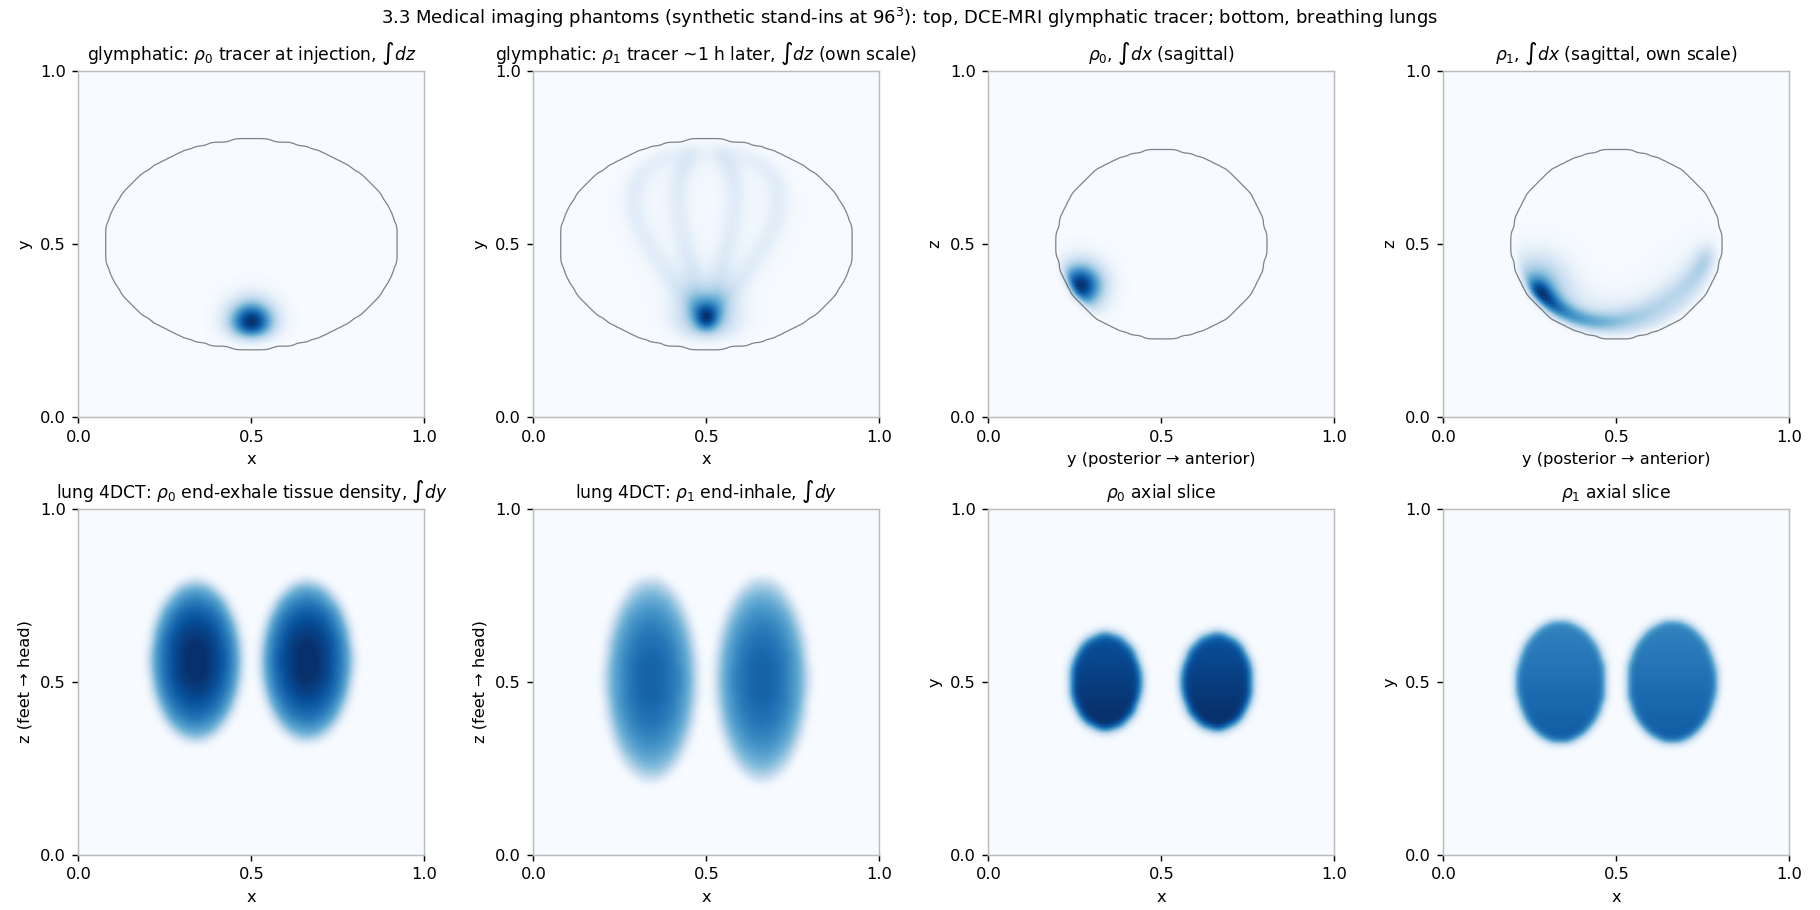
\includegraphics[width=\textwidth]{figures/app_medical.png}
\caption{Medical-imaging phantoms at $96^3$. Top: glymphatic tracer, injected
posteriorly and ventrally ($\rho_0$), then spread along four perivascular channels on
the ventral and lateral brain surface with diffuse parenchymal uptake ($\rho_1$,
drawn on its own colour scale because its peak is $10\times$ lower); the outline is
the brain mask. Bottom: two lung lobes at end-exhale and end-inhale, projected along
the anterior--posterior axis and as an axial slice; the inhale lobes are $25\%$
longer in $z$ and correspondingly less dense.}
\label{fig:appmed}
\end{figure}
\paragraph{Caveats.} Intensities are not conserved mass: lung CT density genuinely
changes with inflation, so mass is not equal; brain MRI intensity is only roughly
proportional to tissue mass. One must renormalize and say so. DIR-Lab lungs are the
most ``mass-like'' (HU tracks tissue density) and have real motion. Skulls and the
table touch the box edges unless masked. Effort: moderate. Paper value: moderate;
expected, and reviewers know unbalanced OT is the honest model here (cite the 2024
unbalanced rOMT).

\subsection{Fluids and geoscience}

\begin{itemize}
  \item JHTDB (\url{https://turbulence.pha.jhu.edu/}), ``Homogeneous buoyancy driven
        turbulence'': $1024^3$ periodic, 1015 frames at $\Delta t=0.04$, stores
        density (Atwood 0.05, Schmidt 1); cutouts via the web / SciServer API. Two
        density frames on a $96^3$ sub-cube give a ``transport a mixing scalar''
        problem. But the field is periodic and the physical evolution is
        advection--diffusion by a turbulent velocity, not OT, so the check is
        qualitative (OT velocity vs.\ DNS velocity at large scales). Here $\eps$ has
        physical meaning (molecular diffusivity $\kappa=\nu/\mathrm{Sc}$) only if the
        domain matches. A dedicated passive-scalar isotropic dataset could not be
        confirmed.
  \item ERA5 pressure levels (Copernicus CDS,
        \url{https://cds.climate.copernicus.eu/datasets/reanalysis-era5-pressure-levels}):
        specific humidity and ozone mass mixing ratio on 37 levels, $0.25^\circ$,
        hourly. The lon-lat-pressure cube is physically non-uniform (air-mass
        weighting, log-pressure vertical) and horizontally periodic; workable for a
        regional box with weak boundary fluxes (a Saharan dust or ozone event), but
        the metric is not Euclidean. Fit: weak, mostly illustrative.
  \item OT data assimilation: Feyeux, Vidard, Nodet, NPG 25:55 (2018), 2D shallow
        water, \url{https://npg.copernicus.org/articles/25/55/2018/}; Bocquet,
        Vanderbecken, Farchi, Dumont Le Brazidec, Roustan, NPG 31:335 (2024),
        ``Bridging classical data assimilation and optimal transport: the 3D-Var
        case'', \url{https://npg.copernicus.org/articles/31/335/2024/}; Farchi,
        Bocquet, Roustan, Mathieu, Qu\'erel, Tellus B 68:31682 (2016), Wasserstein
        comparison of Fukushima radionuclide plumes (public solver at
        \url{http://cerea.enpc.fr/opttrans/}). These are 2D; a 3D plume (FLEXPART /
        Polyphemus output) would be new but requires a model run. Effort: high.
        Paper value: moderate.
\end{itemize}

\paragraph{Can it be run? Yes, 3D for two of the three; the third is 2D.}
Fig.~\ref{fig:appfluid} shows the two 3D stand-ins.
\begin{itemize}
  \item \emph{Atmospheric dispersion (top row).} $\rho_0$ = concentration of a
        pollutant puff just after release, $\rho_1$ = the same puff after time $T$,
        carried downwind and spread by turbulent eddy diffusivity $K$. This is the
        3D version of the Farchi / Bocquet plume comparisons, which were done on
        column-integrated 2D maps. \textbf{$\eps$ has an exact physical meaning}: with
        $\eps=K$ (in box units) the physical evolution is advection--diffusion with a
        uniform wind, the reference process itself has that law, so the SB between
        $\rho_0$ and $\rho_1$ \emph{is} the true plume at every $t$ and $m/\rho$ is the
        wind. This makes the puff a verification problem with a physical $\eps$, and
        it degrades gracefully: a sheared wind gives a plume the SB can only
        approximate, which is the honest version of the data-assimilation use.
        Real plumes have $K_h\gg K_v$; our isotropic $\eps$ is the idealization.
  \item \emph{Buoyancy-driven mixing (bottom row, JHTDB stand-in).} $\rho_0$ = heavy
        fluid fraction with a nearly flat interface, $\rho_1$ = the same scalar after
        plumes have formed. Griddable at $96^3$ from a JHTDB cutout, but the
        physical velocity is divergence-free and turbulent, not a gradient, so the OT
        velocity is at best a large-scale proxy; and a cutout exchanges mass through
        its faces, so renormalization is forced. \textbf{$\eps$ = molecular
        diffusivity $\kappa$} is physical only for the full periodic box. Fit: weak.
  \item \emph{ERA5 humidity / ozone.} 3D (lon, lat, pressure) but on a non-Euclidean,
        air-mass-weighted grid; only a small regional box is a reasonable
        approximation. Illustrative at best; not plotted.
\end{itemize}
\begin{figure}[htbp]\centering
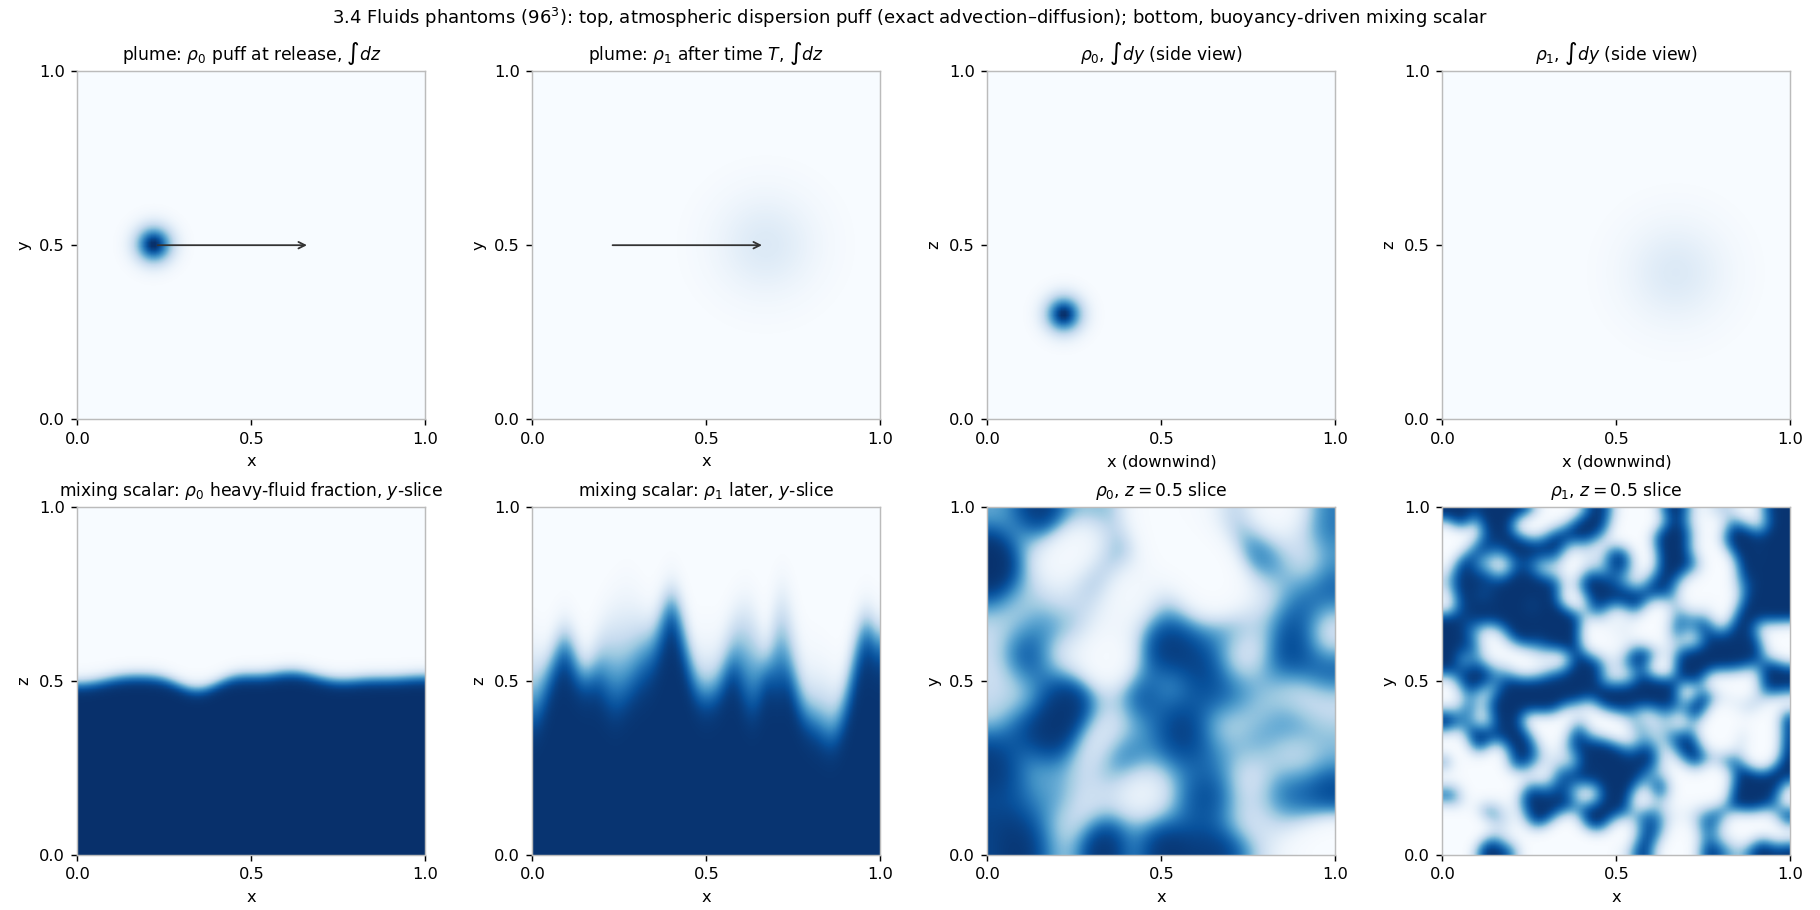
\includegraphics[width=\textwidth]{figures/app_fluids.png}
\caption{Fluids phantoms at $96^3$. Top: a Gaussian puff released at $x=0.22$
($\rho_0$) and the exact advection--diffusion solution after unit time with wind
$(0.45,0,0.12)$ and $K=0.004$ ($\rho_1$), shown integrated along $z$ and along $y$;
the arrow is the wind. Bottom: heavy-fluid fraction before and after mixing, in a
vertical and a horizontal slice.}
\label{fig:appfluid}
\end{figure}

\subsection{Shape interpolation (computer graphics)}

Solomon, de Goes, Peyr\'e, Cuturi, Butscher, Nguyen, Du, Guibas, ``Convolutional
Wasserstein distances'', SIGGRAPH 2015: 3D indicator-function interpolation and
barycenters on $60^3$ and $100^3$ voxel grids, code
\url{https://github.com/gpeyre/2015-SIGGRAPH-convolutional-ot}. Papadakis, Peyr\'e,
Oudet, SIIMS 7:212 (2014), proximal-splitting Benamou--Brenier with obstacles;
released MATLAB code runs 2D+time at $32\times32\times32$,
\url{https://github.com/gpeyre/2013-SIIMS-ot-splitting}. L\'evy, ESAIM M2AN 49:1693
(2015), semi-discrete $L^2$ OT in 3D (tetrahedral meshes, $10^5$--$10^6$ Diracs).
Haber and Horesh, NMTMA 8:97 (2015), multilevel time-dependent OT (3D sizes not
confirmed). Stanford bunny / armadillo / dragon meshes are public (Stanford 3D
Scanning Repository) and voxelize trivially; ShapeNet similar.

Fit: uniform indicator densities are discontinuous (sharp fronts stress positivity;
$\eps$ smooths them), zero at the walls, equal mass after normalization. Reference:
Solomon's convolutional barycenters at matched blur, plus our DCT-Sinkhorn. Effort:
low. Paper value: moderate (familiar to OT reviewers, good figures, shows
$\eps$-smoothing of shocks); the $100^3$ Solomon grid is a natural resolution
comparison point.

\paragraph{Can it be run? Yes, 3D.} $\rho_0$ and $\rho_1$ are the indicator
functions of two voxelized solids, smoothed by one cell and normalized
(Fig.~\ref{fig:appshape}: a torus and a sphere of equal volume, which also changes
topology). Interpretation: $\rho_t$ is the Wasserstein geodesic between the shapes,
the ``morph'' of Solomon et al.; $m/\rho$ is the deformation velocity. \textbf{$\eps$
has no physical meaning.} It is the entropic blur: Solomon's convolutional kernel is
the heat kernel with variance $2\eps$ in our units, so matching their $\gamma$ to our
$\eps$ gives a direct comparison, and the figure to make is the sharpening of the
front as $\eps\to0$.
\begin{figure}[htbp]\centering
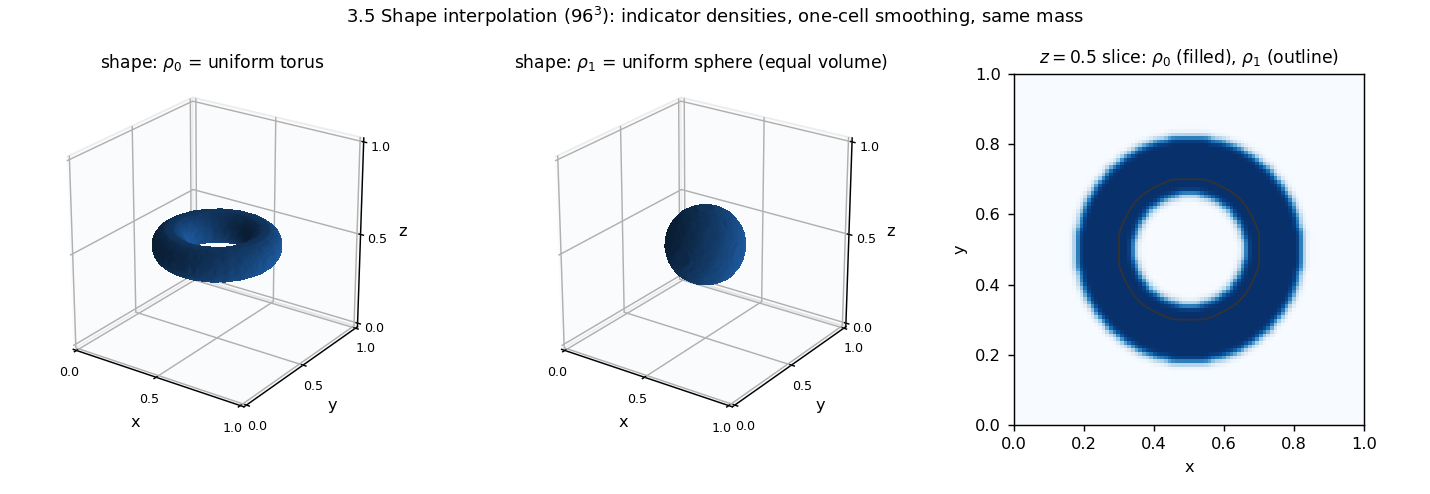
\includegraphics[width=\textwidth]{figures/app_shapes.png}
\caption{Shape-interpolation phantom at $96^3$: a torus ($R=0.24$, $r=0.085$) and a
sphere of the same volume ($r=0.20$), uniform inside, one-cell smoothing, same mass;
right, the mid-plane slice with the sphere's outline over the torus.}
\label{fig:appshape}
\end{figure}

\subsection{Single-cell trajectory inference and density control}

\paragraph{Trajectory inference.} Schiebinger et al., Cell 176:928 (2019),
Waddington-OT: 236k cells, 39 time points (h5ad about 1.4\,GB via CellRank's
\code{reprogramming\_schiebinger}, or \url{https://broadinstitute.github.io/wot/});
Lavenant, Zhang, Kim, Schiebinger, ``Towards a mathematical theory of trajectory
inference'' (2021; Ann.\ Appl.\ Probab.\ 2024): SB with the reference diffusion as
the model, $\eps$ the assumed cell diffusivity. Gridding a 3D PCA / PHATE embedding
(KDE at $64^3$) of day-0 vs.\ day-18 cells gives an SB with a physically motivated
$\eps$, and growth (unbalanced) issues; no published 3D-gridded version was found.
Paper value: moderate, novel; effort moderate; expect reviewers to ask why not the
30-plus intermediate time points (multi-marginal).

\paragraph{Density control.} Chen, Georgiou, Pavon, ``Optimal steering of a linear
stochastic system to a final probability distribution'' I--III, IEEE TAC 2016 / 2018,
and Annual Review of Control 2021, ``Optimal transport in systems and control'': a
swarm of Brownian agents steered between two 3D formations ($\rho_0$ a ring or torus,
$\rho_1$ letters or a cube) with reflecting arena walls is exactly the
Caluya--Halder reflected SB; our solver gives the feedback field $v(t,x)$. Synthetic,
no data needed. Paper value: moderate (the controls audience likes it).

\paragraph{Can they be run? Yes, both in 3D (Fig.~\ref{fig:appcells}).}
\begin{itemize}
  \item \emph{Trajectory inference (top row).} The ``space'' is a 3D embedding of
        gene expression (first three PCA or PHATE coordinates, rescaled to the box),
        so the dimension is three by construction, not by physics. $\rho_0$ = kernel
        density estimate of the day-0 cells, one compact cluster; $\rho_1$ = KDE of
        the day-18 cells: several clusters, one per fate, with unequal weights, plus a
        faint bridge of cells still in transit. Interpretation: $\rho_t$ is the
        inferred population at intermediate days, $m/\rho$ the developmental velocity
        field, and the plan gives fate probabilities per starting cell.
        \textbf{$\eps$ has a model meaning}: Lavenant et al.\ define trajectory
        inference as the SB whose reference diffusion is the cells' stochastic
        gene-expression drift, so $\eps$ is the assumed cell diffusivity in embedding
        coordinates, a parameter to be fitted, not measured. Cell growth and death make
        the honest model unbalanced.
  \item \emph{Density control (bottom row).} A swarm of agents with Brownian noise
        is steered from one formation to another at minimum control energy:
        $\rho_0$ = agents on a ring, $\rho_1$ = agents filling a cube. Reflecting
        arena walls are exactly our Neumann box (Caluya--Halder). Interpretation:
        $v=m/\rho$ is the optimal feedback control law each agent applies at
        $(t,x)$, and $\rho_t$ is the swarm en route. \textbf{$\eps$ has an exact physical
        meaning}: $2\eps=\sigma^2$, the intensity of the agents' noise, i.e.\ how much
        the formation would smear if uncontrolled. Synthetic by nature, so no data
        issue at all.
\end{itemize}
\begin{figure}[htbp]\centering
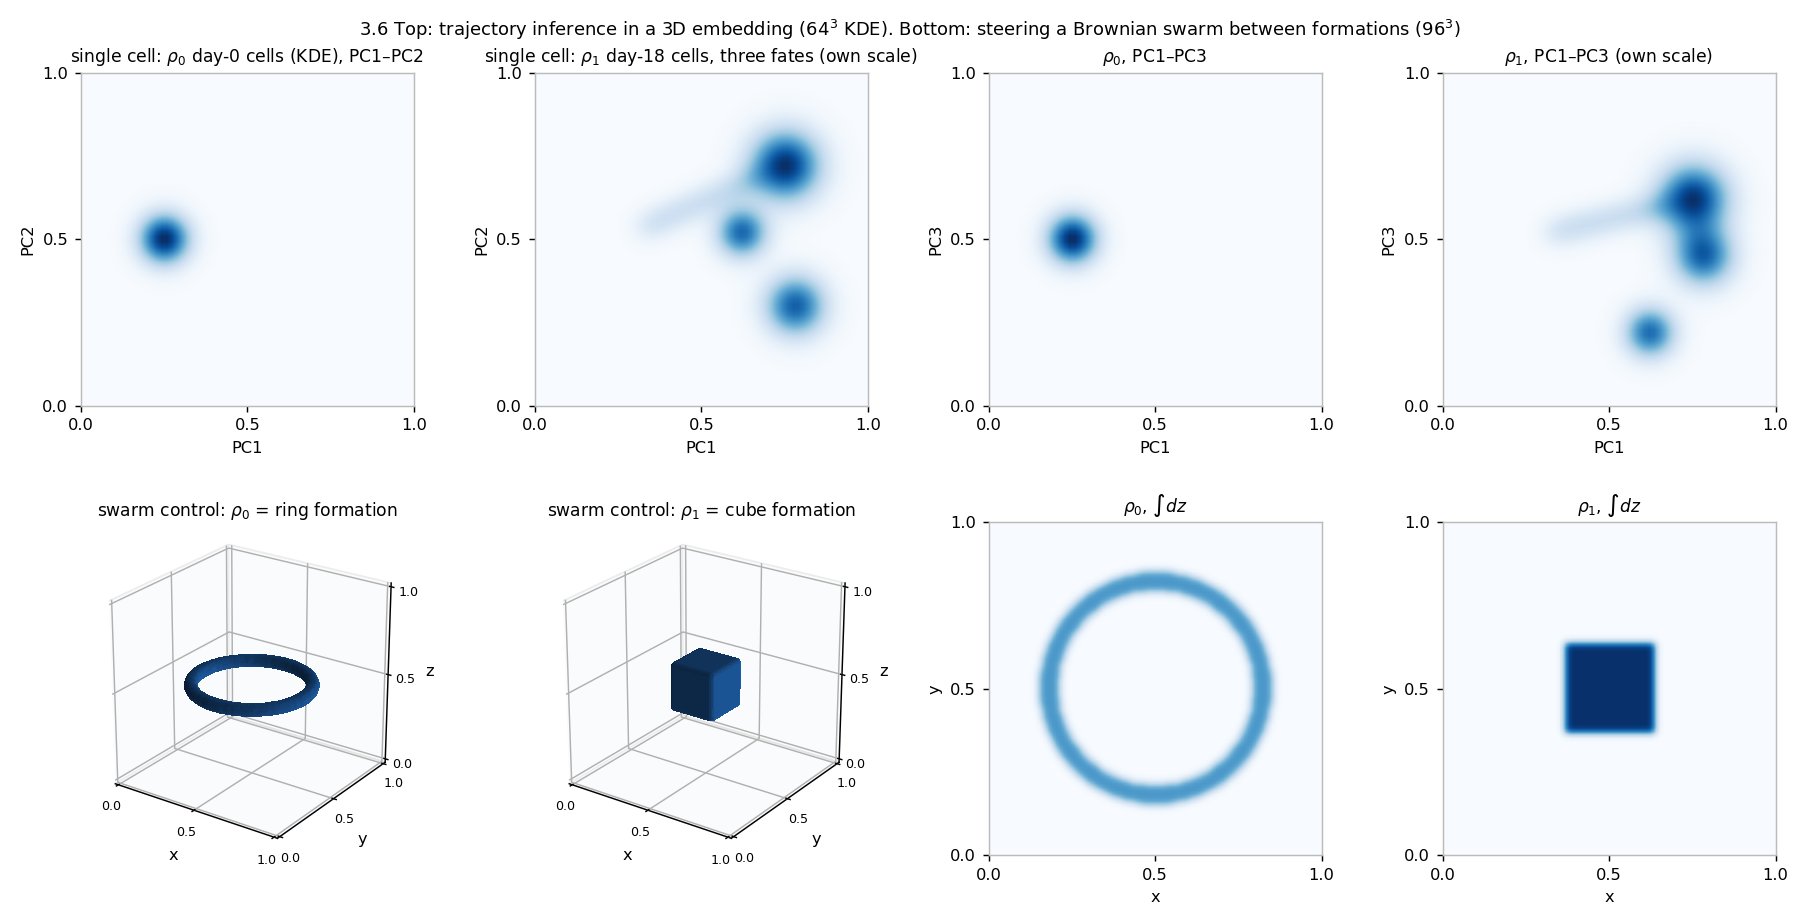
\includegraphics[width=\textwidth]{figures/app_cells_control.png}
\caption{Top: trajectory-inference phantom on a $64^3$ embedding grid, day-0 cells
and day-18 cells with three fates of weights $0.5/0.3/0.2$ and a transit bridge,
projected onto two coordinate planes ($\rho_1$ on its own colour scale). Bottom:
swarm control at $96^3$, a ring formation and a cube formation, as isosurfaces and
integrated along $z$.}
\label{fig:appcells}
\end{figure}

\paragraph{Summary of Secs.~3.2--3.6.}
\begin{center}\small
\begin{tabular}{llll}\toprule
problem & grid & $\rho_0\to\rho_1$ & meaning of $\eps$\\\midrule
cryo-EM conformations & 3D & closed $\to$ open map & map resolution (blur), MorphOT's $\gamma$\\
glymphatic DCE-MRI & 3D & tracer early $\to$ late & tracer diffusivity (physical, tiny)\\
lung 4DCT & 3D & tissue density exhale $\to$ inhale & none (regularizer)\\
dispersion puff & 3D & release $\to$ downwind & eddy diffusivity $K$ (exact)\\
JHTDB mixing cutout & 3D & interface $\to$ plumes & molecular $\kappa$ (full box only)\\
plume assimilation (Farchi) & 2D & column maps & eddy diffusivity (heuristic)\\
ERA5 ozone / humidity & 3D, non-Euclidean & regional box & none\\
shape morphing & 3D & torus $\to$ sphere & entropic blur (Solomon's $\gamma$)\\
trajectory inference & 3D embedding & day 0 $\to$ day 18 & cell diffusivity (model parameter)\\
swarm density control & 3D & ring $\to$ cube & agent noise $\sigma^2/2$ (exact)\\
\bottomrule
\end{tabular}
\end{center}

\section{Ranked shortlist}
\label{sec:shortlist}

\begin{enumerate}[leftmargin=1.8em, itemsep=3pt]
  \item \textbf{Anisotropic / unequal-covariance Gaussians} (Bunne 2023, Janati
        2020), including the self-bridge $\rho_0=\rho_1$: mandatory verification;
        cost, $\rho_t$ and $m$ all closed form. [verification]
  \item \textbf{Gushchin-style LSE mixture pairs in 3D} (multimodal, exact drift,
        $\rho_1$ by quadrature) plus the product-of-1D bridges; DCT-Sinkhorn as the
        grid-exact reference for everything else. [verification]
  \item \textbf{Cryo-EM: EMD-5137 $\to$ EMD-5139} (Mm-cpn closed $\to$ open) at
        $64$--$96^3$, compared with MorphOT's entropic barycenters. [application;
        best box / no-flux fit]
  \item \textbf{Cosmology: CAMELS CMD $128^3$ $M_{\rm tot}$ grids}, $z=1$ (or
        uniform) $\to z=0$ on a padded sub-cube, with displacement-field checks
        against the Lagrangian truth or L\'evy's semi-discrete MAK; explicitly
        discuss periodic vs.\ no-flux and $\eps$ as a heuristic velocity-dispersion
        smoothing. [application; highest narrative value]
  \item \textbf{Lung 4DCT} (DIR-Lab, end-exhale $\to$ end-inhale) with
        landmark-based checks, framed as approximately balanced; cite rOMT
        (Chen / Tannenbaum 2023--24) as the closest prior 3D advection--diffusion OT.
        [application]
  \item \textbf{3D shape interpolation} (Stanford bunny $\to$ armadillo at
        $64$--$100^3$) replicating Solomon et al.\ 2015 resolutions, showing
        $\eps$-smoothing of fronts. [application / benchmark]
\end{enumerate}

\paragraph{Where $\eps$ is physical.} Glymphatic / tracer rOMT (diffusivity);
buoyancy or passive-scalar turbulence (molecular diffusivity, only with matching
boundary conditions); single-cell SB (cell-state diffusivity in Lavenant et al.);
swarm steering (agent noise). In cosmology and cryo-EM it is a regularization or blur
(MorphOT's $\gamma$), not a physical constant; no SB-cosmology paper was found, so any
``velocity dispersion'' reading should be presented as a heuristic.

\section*{Key links}
\begin{itemize}
  \item arXiv 2202.05722 (Bunne), 2006.02572 (Janati), 2006.03416 (Mallasto),
        2306.10161 (Gushchin; \url{https://github.com/ngushchin/EntropicOTBenchmark}),
        2003.13895 (Caluya--Halder).
  \item CAMELS CMD \url{https://camels-multifield-dataset.readthedocs.io};
        Quijote \url{https://quijote-simulations.readthedocs.io/en/latest/df.html}.
  \item EMDB \url{https://www.ebi.ac.uk/emdb/} (EMD-5137 / 5139; Nature 463:379);
        MorphOT bioRxiv 10.1101/2020.09.08.286302 and AIMS Math 7(1) 2022 (PMC9377683).
  \item DIR-Lab \url{https://www.dir-lab.com/}; Learn2Reg
        \url{https://learn2reg.grand-challenge.org/}; BrainWeb
        \url{https://brainweb.bic.mni.mcgill.ca/}; rOMT Sci.\ Rep.\
        \url{https://www.nature.com/articles/s41598-023-50874-y}.
  \item JHTDB \url{https://turbulence.pha.jhu.edu/}; ERA5
        \url{https://cds.climate.copernicus.eu/datasets/reanalysis-era5-pressure-levels};
        Bocquet et al.\ 2024 \url{https://npg.copernicus.org/articles/31/335/2024/};
        Feyeux et al.\ 2018 \url{https://npg.copernicus.org/articles/25/55/2018/}.
  \item Solomon et al.\ code \url{https://github.com/gpeyre/2015-SIGGRAPH-convolutional-ot};
        WOT \url{https://broadinstitute.github.io/wot/}.
\end{itemize}

\end{document}
